\section{Eksperymenty}
Celem przetestowania wybranych metod XAI powstał plan eksperymentów dla każdego ze zbiorów. Jest on następujący:
\begin{enumerate}
    \item przeanalizować zbiór danych, w tym ocenić ilość wartości brakujących, znaleźć kolumny jakościowe;
    \item przetworzyć dane, na co składa się m.in. uzupełnienie braków czy kodowanie zmiennych jakościowych;
    \item zapisać przerobione dane w celu ułatwienia ich wykorzystania w przyszłości;
    \item znormalizować zbiór i podzielić go na podzbiory - treningowy i testowy;
    \item stworzyć model, nauczyć go na zbiorze treningowym i ocenić zbiorem testowym;
    \item dla każdej metody XAI:
    \begin{enumerate}
        \item poddać model analizie poprzez metodę XAI;
        \item przeanalizować otrzymane wyniki;
    \end{enumerate}
    \item powtórzyć punkty 5. i 6. dla reszty modeli.
\end{enumerate}
W przypadku danych zdjęciowych dodatkowo pomiędzy podzieleniem zbioru a nauką pierwszego modelu dochodzi do wybrania badanej próbki, którą ów model przed zostaniem poddanym analizie klasyfikuje.

\subsection{Diabetes Prediction}
Jak wskazuje Tabela \ref{tab:metrics_diabetes} \textbf{las losowy} osiągnął dokładność na poziomie 72\%. Ze względu na równy rozkład próbek przynależących do poszczególnych klas decyzyjnych średnie arytmetyczne oraz ważone tej miary były jednakowe. Z 500 przypadków niebędących diabetykami model dobrze rozpoznał 352, co skutkuje specyficznością równą 70\%. Mając do dyspozycji same próbki osób chorujących na cukrzycę model poprawnie zaklasyfikował 367 przypadków. Precyzja osiągnęła poziom 71\%, czułość 73\% a F1-score 72\%. Pole powierzchni pod krzywą ROC wyliczone zostało w przybliżeniu na 0.79. 

W przypadku \textbf{XGBoost'a} prawie wszystkie przedstawione miary wyniosły 70\%. Jedynie ROC AUC i czułość różniły się, gdzie w pierwszym przypadku model osiągnął 0.77, a drugim 0.69. Rozkład prawidłowych i błędnych predykcji są bardzo zbliżone. Jako klasa '0' zostało zdiagnozowanych 5 próbek więcej niż do jej alternatywy. 

Wybrana za pomocą przeszukiwania określonej przestrzeni hiperparametrów \textbf{sieć neuronowa} składa się z warstw ukrytych w postaci 64-64 neuronów, używa funkcji aktywacji tanh, mechanizm \textit{Early Stopping}'u oraz optymalizator Adam. Osiągnięta przez nią dokładność wyniosła 72\%, a ROC AUC 0.8. Model częściej zaliczał próbkę jako diabetyka. Znacznie skutecnziej identyfikował tę klasę - o 21 poprawnych przypadków więcej w porównaniu do wyboru alternatywnego. 

\begin{xltabular}{\textwidth}{|c|>{\centering\arraybackslash}X|c|c|c|c|c|}
\caption{Wyniki metryk poszczególnych modeli dla zbioru dotyczącego diabetyków}
\label{tab:metrics_diabetes}\\
\hline
Model \textbackslash Metryka & ROC AUC & Precyzja & Czułość & Specyficzność & F1-score & Dokładność \\ \hline
\endfirsthead
Random Forest & 0.79 & 0.71 & 0.73 & 0.70 & 0.72 & 0.72 \\ \hline
XGBoost & 0.77 & 0.70 & 0.69 & 0.70 & 0.70 & 0.70 \\ \hline
Sieć neuronowa & 0.80 & 0.71 & 0.74 & 0.70 & 0.72 & 0.72 \\ \hline
\end{xltabular}

\subsubsection{Random Forest}
Z wykresu znajdującego się na Rys. \ref{fig:lime_absolutemeanplot_rf_diabetes} widzimy, że najistotniejszą informacją wpływającą na predykcje według \textbf{LIME} jest ,,HvyAlcoholConsump'', której obliczona miara wyniosła ok. 0.16. Kolejną znaczną przesłanką jest ,,GenHlth'' z wynikiem w przybliżeniu 0.13. ,,Age'', ,,BMI'', ,,HeartDiseaseorAttack'' i ,,DiffWalk'' należą do kolejnych przydatnych cech, których wagi oscylują w przedziale od 0.05 do 0.1. Informacjami bez jakichkolwiek wartości okazały się być: ,,Veggies'', ,,CholCheck'' oraz ,,AnyHealthcare''. 

\begin{figure}[H]
    \centering
    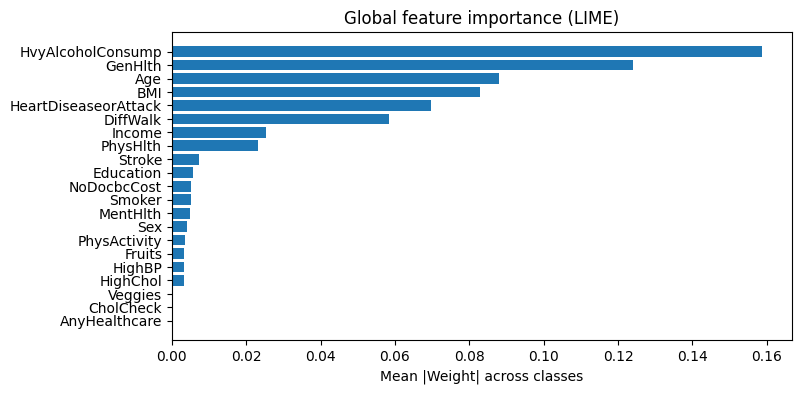
\includegraphics[width=0.9\linewidth]{rysunki/diabetes/lime_absolutemeanplot_rf_diabetes.png}
    \caption{Wykres średnich obliczonych z bezwzględnych wartości wag LIME modelu Random Forest zbioru dotyczącego diabetyków [źródło własne]}
    \label{fig:lime_absolutemeanplot_rf_diabetes}
\end{figure}

Z Rys. \ref{fig:shap_absolutemeanplot_rf_diabetes} można wyczytać, że za najważniejszą cechę predykcyjną metoda \textbf{SHAP} uznała ,,GenHlth'' zmieniającą średnio przewidywanie o ok. 9\%. Zaraz po w rankingu istotności znajduje się ,,HighBP'' z miarą bardzo zbliżoną do pierwszej zmiennej. Na trzecim miejscu znalazło się ,,BMI'' wpływające na prawdopodobieństwo diagnozy w przybliżeniu o 7\%. Tutaj również zauważamy, iż aż 12 cech miało znikome znaczenie. Ich suma przedstawiona na dole wykresu wyniosła raptem 11\%, co średnio każdej z poszczególnych zmiennych daje mniej niż 1\% istotności. Ponownie do owych cech zaliczamy kolumny: ,,Fruits'', ,,Veggies'', ,,Smoker'' czy ,,Stroke''.

\begin{figure}[H]
    \centering
    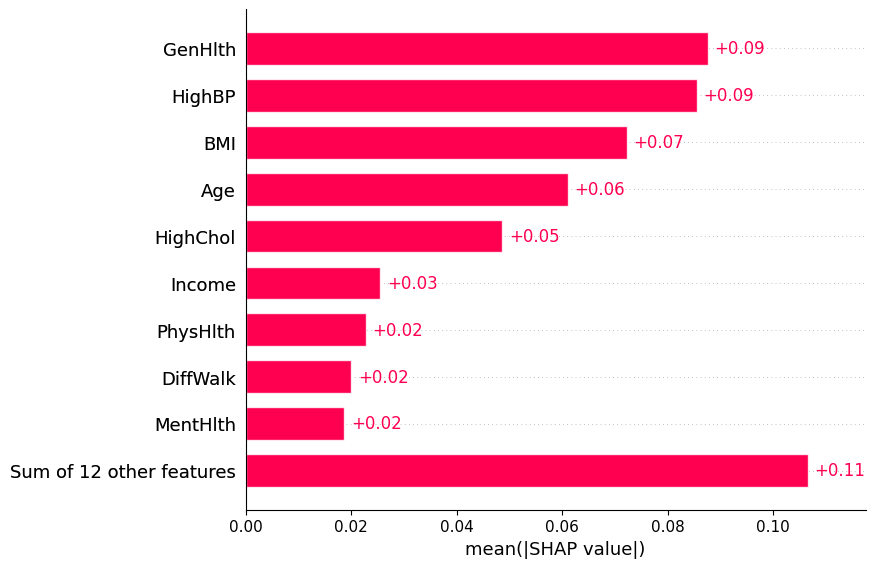
\includegraphics[width=0.75\linewidth]{rysunki/diabetes/shap_absolutemeanplot_rf_diabetes.png}
    \caption{Wykres średnich obliczonych z bezwzględnych wartości SHAP modelu Random Forest zbioru dotyczącego diabetyków [źródło własne]}
    \label{fig:shap_absolutemeanplot_rf_diabetes}
\end{figure}

,,GenHlth'', ,,HighBP'' oraz ,,Age'' charakteryzowały się tym, że ich wysokie wartości miały mniejsze znaczenie, na wizualizacji przedstawionej na Rys. \ref{fig:shap_beeswarm_rf_diabetes} występują pośrodku, mniej więcej od -1\% do +2\%. Natomiast niskie osiągi miały znacznie wyraźniejsze przesłanie, za czym przemawia ich rozłożenie na krańcach odpowiadających wierszy. Oznacza to, że niska ocena stanu zdrowia, nieposiadanie wysokiego ciśnienia krwi oraz bycie młodym zmniejszają lub zwiększają w zauważalnym stopniu prawdopodobieństwo chorowania oraz nieprzejawiania cukrzycy. Są to zupełnie przeciwne wyniki. Podobna sytuacja ma miejsce w przypadku ,,DiffWalk'' i ,,MentHlth'', gdzie na brzegach widnieją czerwone kropki, a pomiędzy nimi niebieskie. Wartości trzeciej najistotniejszej cechy - ,,BMI'' są przemieszane, niewskazując na jakąś ogólną zależność.

\begin{figure}[H]
    \centering
    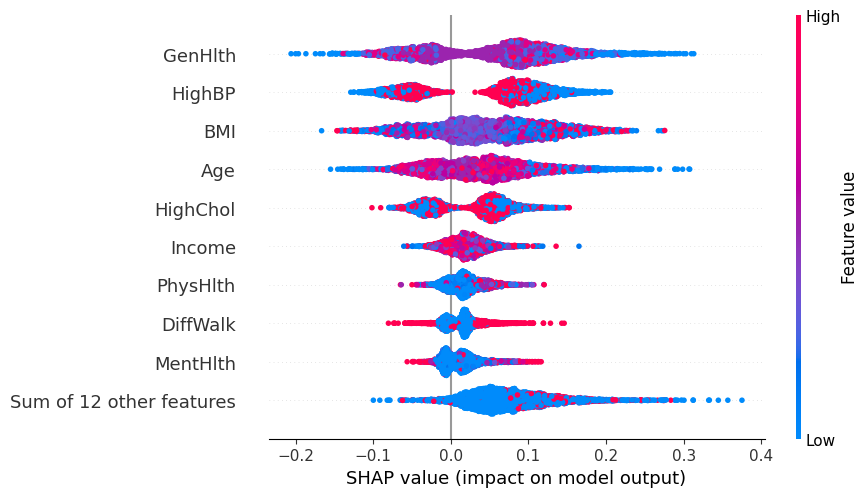
\includegraphics[width=1\linewidth]{rysunki/diabetes/shap_beeswarm_rf_diabetes.png}
    \caption{Wykres typu ,,beeswarm'' wartości SHAP modelu Random Forest zbioru dotyczącego diabetyków [źródło własne]}
    \label{fig:shap_beeswarm_rf_diabetes}
\end{figure}


\begin{xltabular}{\textwidth}{|c|c|c|}
    \caption{Wyniki uzyskane po użyciu metody PFI przy modelu Random Forest dla zbioru dotyczącego diabetyków}
    \label{tab:pfi_rf_diabetes}\\ \hline
    Cecha & Średnia & Odchylenie standardowe \\ \hline
    \endfirsthead

    GenHlth              & 0.146 &  0.005 \\ \hline
    BMI                  & 0.143 &  0.004 \\ \hline
    HighBP               & 0.115 &  0.003 \\ \hline
    Age                  & 0.109 &  0.003 \\ \hline
    HighChol             & 0.072 &  0.003 \\ \hline
    Income               & 0.059 &  0.002 \\ \hline
    PhysHlth             & 0.051 &  0.002 \\ \hline
    MentHlth             & 0.037 &  0.002 \\ \hline
    Education            & 0.031 &  0.002 \\ \hline
    Sex                  & 0.027 &  0.001 \\ \hline
    DiffWalk             & 0.027 &  0.001 \\ \hline
    HeartDiseaseorAttack & 0.024 &  0.002 \\ \hline
    Smoker               & 0.023 &  0.001 \\ \hline
    Fruits               & 0.017 &  0.001 \\ \hline
    PhysActivity         & 0.014 &  0.001 \\ \hline
    Veggies              & 0.009 &  0.001 \\ \hline
    HvyAlcoholConsump    & 0.008 &  0.001 \\ \hline
    Stroke               & 0.006 &  0.000 \\ \hline
    NoDocbcCost          & 0.004 &  0.000 \\ \hline
    CholCheck            & 0.004 &  0.001 \\ \hline
    AnyHealthcare        & 0.003 &  0.000 \\ \hline
\end{xltabular}

Jak pokazuje wykres znajdujący się na Rys. \ref{fig:pfi_rf_diabetes} metoda \textbf{PFI} wskazała wszystkie cechy za istotne w przewidywaniu. Z Tabeli \ref{tab:pfi_rf_diabetes} możemy wyczytać, że najważniejszą z nich okazała się być ,,GenHlth'' średnio zmieniająca dokładność o 14.6\% z odchyleniem standardowym  0.005. Cechą o bardzo zbliżonym wyniku jest ,,BMI'', którego permutacja zmniejsza miarę o 14.3\%, przy odchyleniu standardowym 0.004. Na trzecim miejscu plasuje się ,,HighBP'' z wynikiem od 11.2\% do 11.8\%. Najmniej informacji niosły za sobą ,,NoDocbcCost'', ,,CholCheck'' oraz ,,AnyHealthcare''. Wartości owych zmiennych oscylowały w granicach ok. 0.4\% - 0.3\%.

\begin{figure}[H]
    \centering
    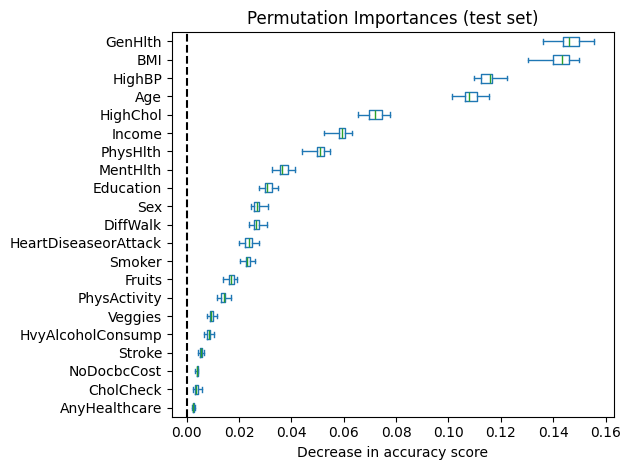
\includegraphics[width=0.75\linewidth]{rysunki/diabetes/pfi_rf_diabetes.png}
    \caption{Wykres pudełkowy pokazujący wpływ cech na predykcję uzyskany po użyciu metody PFI przy modelu Random Forest dla zbioru dotyczącego diabetyków [źródło własne]}
    \label{fig:pfi_rf_diabetes}
\end{figure}

\subsubsection{XGBoost}
Z Rys. \ref{fig:lime_absolutemeanplot_xgb_diabetes} możemy wyczytać, że za najistotniejszą cechę \textbf{LIME} uznało ,,HighBP'' z miarą ponad 0.16. Trochę mniej wartościową informację wnosi ,,Income'' z wynikiem ok. 0.13, a zaraz po nim znajduje się ,,BMI'' osiągające w przybliżeniu wartość 0.11. W ogóle nieprzydatne okazały się być zmienne: ,,Veggies'', ,,CholCheck'' oraz ,,AnyHealthcare''.

\begin{figure}[H]
    \centering
    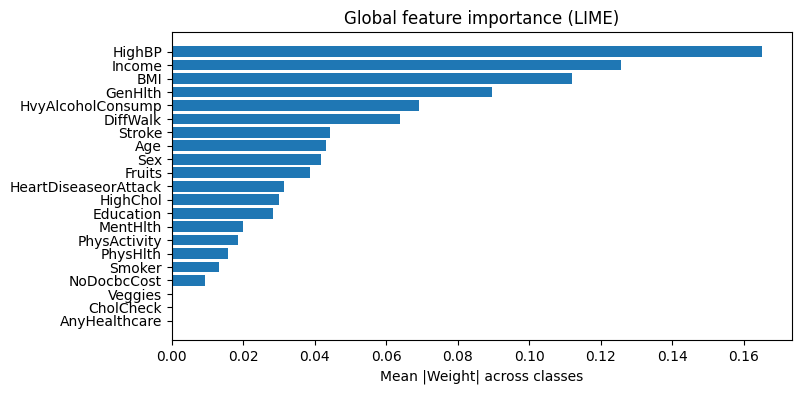
\includegraphics[width=0.9\linewidth]{rysunki/diabetes/lime_absolutemeanplot_xgb_diabetes.png}
    \caption{Wykres średnich obliczonych z bezwzględnych wartości wag LIME modelu XGBoost zbioru dotyczącego diabetyków [źródło własne]}
    \label{fig:lime_absolutemeanplot_xgb_diabetes}
\end{figure}

Wykres zaprezentowany na Rys. \ref{fig:shap_absolutemeanplot_xgb_diabetes} pokazuje, iż najistotniejszy wpływ na wynik przewidywania według metody \textbf{SHAP} miało ,,GenHlth'' z wartością 0.73, następnie było to ,,BMI'' z wynikiem 0.57, a na 3 miejscu ex aequo wiek ,,Age'' oraz informacja o wysokim ciśnieniu krwi ,,HighBP'' z miarą 0.55. Wśród 12 najmniej znaczących cech znalazło się m.in.: ,,Veggies'', ,,Fruits'', ,,HvyAlcoholConsump'', ,,Sex'' i ,,Smoker''.

\begin{figure}[H]
    \centering
    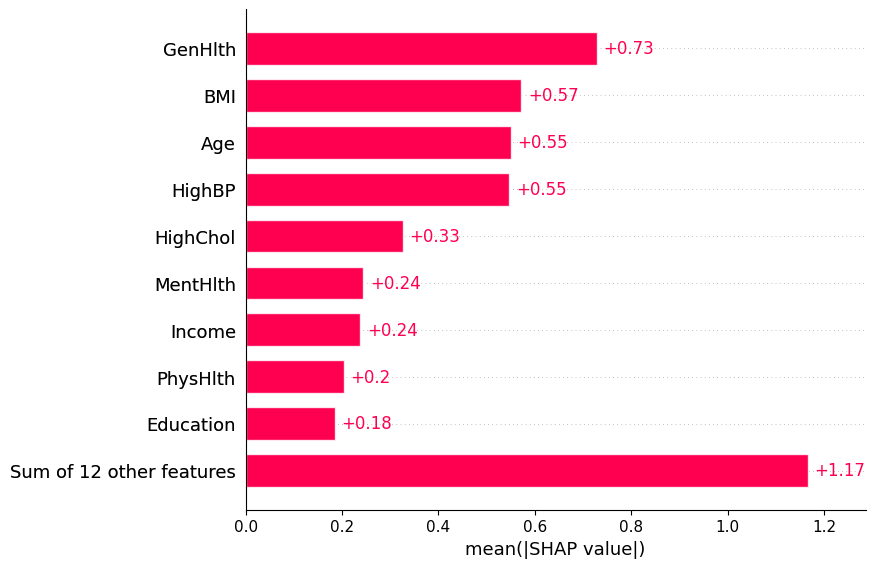
\includegraphics[width=0.75\linewidth]{rysunki/diabetes/shap_absolutemeanplot_xgb_diabetes.png}
    \caption{Wykres średnich obliczonych z bezwzględnych wartości SHAP modelu XGBoost zbioru dotyczącego diabetyków [źródło własne]}
    \label{fig:shap_absolutemeanplot_xgb_diabetes}
\end{figure}

Wykres typu ,,rój pszczół'' zamieszczony na Rys. \ref{fig:shap_beeswarm_xgb_diabetes} pokazuje bardzo wyraźne zależności pomiędzy wartościami cech a wartościami uzyskanymi poprzez metodę SHAP. Kropki odpowiadające niskim liczbom pięciu najważniejszych cech, czyli ,,GenHlth'', ,,BMI'', ,,Age'', ,,HighBP'' oraz ,,HighChol'', zostały narysowane po lewej stronie, co oznacza, że zmniejszają one \textit{log odds}. Ich fioletowe punkty mieszczą się wokół 0, natomiast czerwone - przeważnie znajdują się po prawej, przemawiając za ich dodatnim wpływem. Wynika z tego, że zła ocena własnego zdrowia, małe BMI, bycie młodym, posiadanie niskiego cholesterolu oraz ciśnienia krwi przyczyniają się do zaklasyfikowania jako osoba zdrowa. Logiczniej byłoby przypuszczać, iż wyniki uzyskane dla 'GenHlth' powinny być odwrotne - to wysoka ocena swojego stanu zdrowia powinna świadczyć o nie byciu diabetykiem. Dla reszty cech punkty są przemieszane, nie oferując zbyt wartościowego wglądu w badaną korelację.     

\begin{figure}[H]
    \centering
    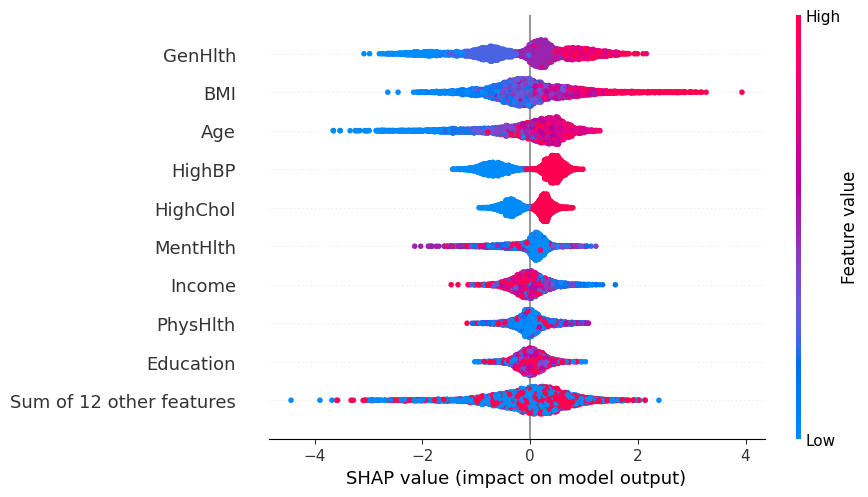
\includegraphics[width=1\linewidth]{rysunki/diabetes/shap_beeswarm_xgb_diabetes.png}
    \caption{Wykres typu ,,beeswarm'' wartości SHAP modelu XGBoost zbioru dotyczącego diabetyków [źródło własne]}
    \label{fig:shap_beeswarm_xgb_diabetes}
\end{figure}

\begin{xltabular}{\textwidth}{|c|c|c|}
    \caption{Wyniki uzyskane po użyciu metody PFI przy modelu XGBoost dla zbioru dotyczącego diabetyków}
    \label{tab:pfi_xgb_diabetes}\\ \hline
    Cecha & Średnia & Odchylenie standardowe \\ \hline
    \endfirsthead
    BMI                  & 0.149 &  0.004 \\ \hline
    Age                  & 0.128 &  0.004 \\ \hline
    GenHlth              & 0.126 &  0.003 \\ \hline
    Income               & 0.085 &  0.003 \\ \hline
    PhysHlth             & 0.063 &  0.004 \\ \hline
    Education            & 0.055 &  0.002 \\ \hline
    MentHlth             & 0.055 &  0.002 \\ \hline
    HighBP               & 0.049 &  0.003 \\ \hline
    HighChol             & 0.034 &  0.002 \\ \hline
    Smoker               & 0.028 &  0.002 \\ \hline
    Sex                  & 0.025 &  0.002 \\ \hline
    Fruits               & 0.024 &  0.002 \\ \hline
    PhysActivity         & 0.023 &  0.002 \\ \hline
    DiffWalk             & 0.019 &  0.002 \\ \hline
    Veggies              & 0.019 &  0.002 \\ \hline
    HeartDiseaseorAttack & 0.017 &  0.002 \\ \hline
    HvyAlcoholConsump    & 0.015 &  0.002 \\ \hline
    CholCheck            & 0.010 &  0.001 \\ \hline
    NoDocbcCost          & 0.009 &  0.001 \\ \hline
    Stroke               & 0.008 &  0.001 \\ \hline
    AnyHealthcare        & 0.004 &  0.001 \\ \hline
\end{xltabular}

Jak podaje wykres na Rys. \ref{fig:pfi_xgb_diabetes} według metody \textbf{PFI} permutacja którejkolwiek z cech powoduje spadek w dokładności modelu. Największy ma miejsce przy zmianie ,,BMI'' i wynosi średnio 14.9\% z odchyleniem standardowym rzędu 0.004. Kolejną cechą o dużym znaczeniu jest ,,Age'' z miarą 12.8\% i granicą 0.004. Zaraz po nim znajduje się ,,GenHlth'' z wynikiem od 12.3\% do 12.9\%. Jak czytamy w Tabeli \ref{tab:pfi_xgb_diabetes} trzy ostatnie zmienne nie wpływają na dokładność o więcej niż 1\%, a są to: ,,NoDocbcCost'', ,,Stroke'' oraz ,,AnyHealthcare''.

\begin{figure}[H]
    \centering
    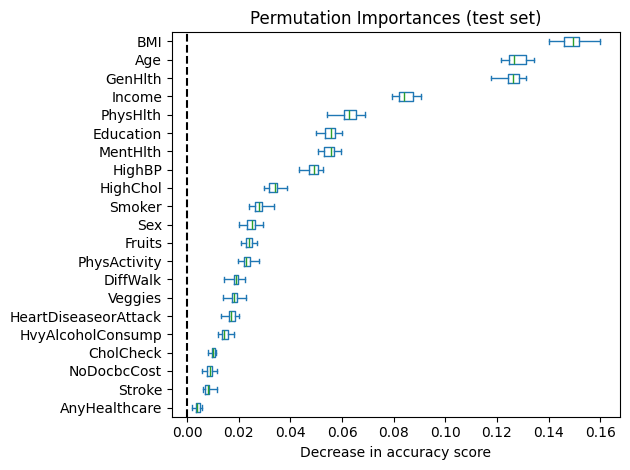
\includegraphics[width=0.75\linewidth]{rysunki/diabetes/pfi_xgb_diabetes.png}
    \caption{Wykres pudełkowy pokazujący wpływ cech na predykcję uzyskany po użyciu metody PFI przy modelu XGBoost dla zbioru dotyczącego diabetyków [źródło własne]}
    \label{fig:pfi_xgb_diabetes}
\end{figure}

\subsubsection{Sieć neuronowa}
Na Rys. \ref{fig:lime_absolutemeanplot_dnn_diabetes} zauważamy w rozumowaniu \textbf{LIME} dużą przewagę wartości predykcyjnej cechy ,,HvyAlcoholConsump''. Jej waga znacznie przekracza 0.2, wskazując jak silną wnosi informację. Kolejną informacją w rankingu istotności jest ,,GenHlth'' z wartością trochę mniejszą niż 0.175. Tuż za nią plasuje się ,,BMI'' z wynikiem ok. 0.14. Ostatnią cechą będącą nie 2-krotnie mniej wartościową od tej najważniejszej jest ,,Age''. Brak jakiegokolwiek znaczenia miały: ,,Veggies'', ,,CholCheck'' oraz ,,AnyHealthcare''.   

\begin{figure}[H]
    \centering
    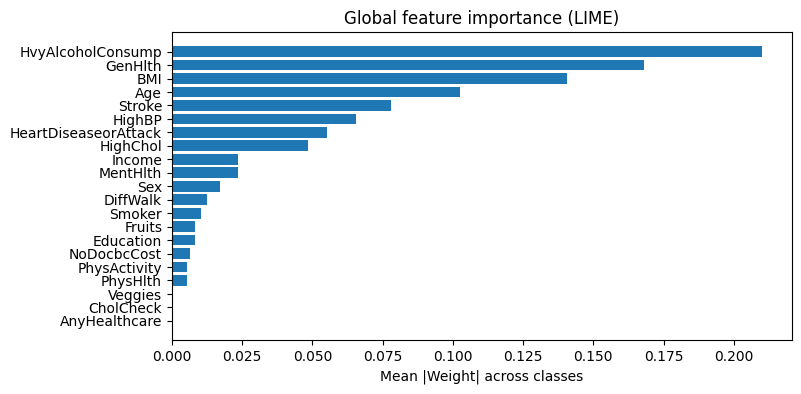
\includegraphics[width=0.9\linewidth]{rysunki/diabetes/lime_absolutemeanplot_dnn_diabetes.png}
    \caption{Wykres średnich obliczonych z bezwzględnych wartości wag LIME modelu sieci neuronowej zbioru dotyczącego diabetyków [źródło własne]}
    \label{fig:lime_absolutemeanplot_dnn_diabetes}
\end{figure}

Na Rys. \ref{fig:shap_absolutemeanplot_dnn_diabetes} zauważamy, że \textbf{SHAP} największą wartość predykcyjną przypisał cesze ,,GenHlth'', wpływającej na prawdopodobieństwo konkretnej klasyfikacji o 10\%. Kolejną ważną informacją pod względem istotności jest ,,BMI'' zmieniające szansę diagnozy o 8\%, a zaraz po niej znajduje się ,,HighBP'' z wartością 7\%. Wśród tych najmniej znaczących zmiennych znalazło się wykształcenie ,,Education'' czy palenie papierosów ,,Smoker''. 12 najgorszych zmiennych w owej klasyfikacji osiągnęły istotność nie większą niż 1\%.

\begin{figure}[H]
    \centering
    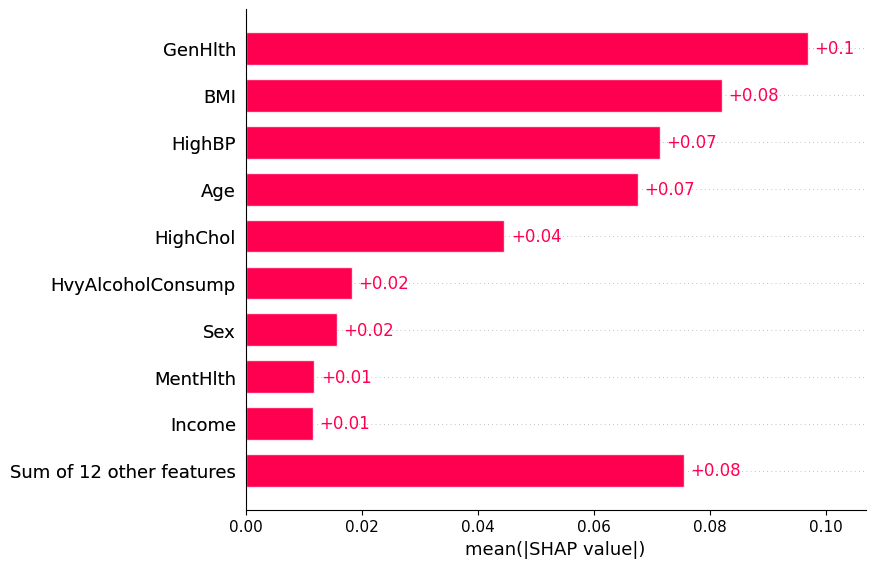
\includegraphics[width=0.75\linewidth]{rysunki/diabetes/shap_absolutemeanplot_dnn_diabetes.png}
    \caption{Wykres średnich obliczonych z bezwzględnych wartości SHAP modelu sieci neuronowej zbioru dotyczącego diabetyków [źródło własne]}
    \label{fig:shap_absolutemeanplot_dnn_diabetes}
\end{figure}

Analizując wykres zamieszczony na Rys. \ref{fig:shap_beeswarm_dnn_diabetes} zauważamy, że wskazuje on na parę istotnych zależności. Średnie wartości: ,,GenHlth'', ,,BMI'' oraz ,,Age'' mają nie za duży wpływ na przewidywanie modelu. Wysokie liczby w kolumnach odpowiadających ,,HvyAlcoholConsump'', ,,MentHlth'' i ,,BMI'' mieszczą się na skrajach wierszy pokazując ich znaczny wpływ na klasyfikację. Odwrotna sytuacja ma miejsce w przypadku: ,,HighBP'', ,,HighChol'', a także ,,Income''; gdzie to niebieskie punkty są na brzegach. Oznacza to, że we wskazanych cechach ich niskie bądź wysokie wartości przemawiają za byciem lub nie diabetykiem, co sobie przeczy.  

\begin{figure}[H]
    \centering
    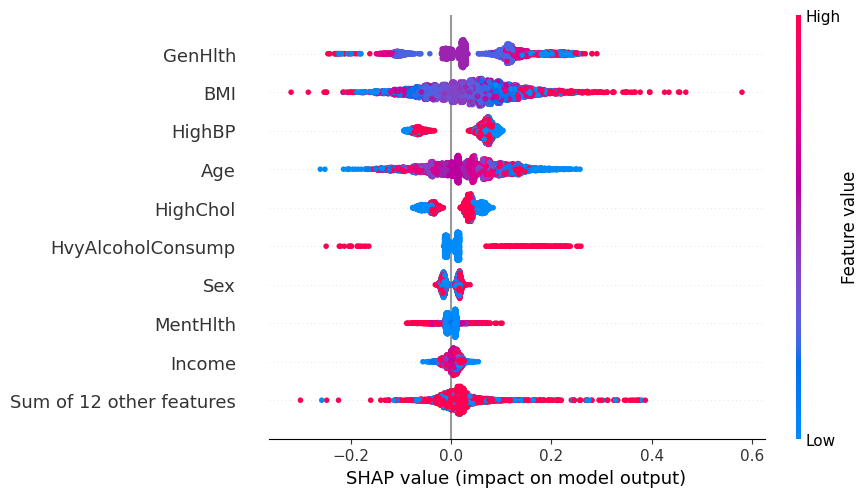
\includegraphics[width=1\linewidth]{rysunki/diabetes/shap_beeswarm_dnn_diabetes.png}
    \caption{Wykres typu "'beeswarm"' wartości SHAP modelu sieci neuronowej zbioru dotyczącego diabetyków [źródło własne]}
    \label{fig:shap_beeswarm_dnn_diabetes}
\end{figure}


\begin{xltabular}{\textwidth}{|c|c|c|}
    \caption{Wyniki uzyskane po użyciu metody PFI przy modelu sieci neuronowej dla zbioru dotyczącego diabetyków}
    \label{tab:pfi_dnn_diabetes}\\ \hline
    Cecha & Średnia & Odchylenie standardowe \\ \hline
    \endfirsthead
    GenHlth           & 0.055 &  0.006 \\ \hline
    BMI               & 0.041 &  0.004 \\ \hline
    Age               & 0.023 &  0.003 \\ \hline
    HighBP            & 0.021 &  0.003 \\ \hline
    HvyAlcoholConsump & 0.007 &  0.002 \\ \hline
    CholCheck         & 0.006 &  0.002 \\ \hline
\end{xltabular}

Jak podaje Tabela \ref{tab:pfi_dnn_diabetes} z 21 cech \textbf{PFI} wskazało tylko 6, których permutacja zawsze miała negatywny wpływ na dokładność. Największe znaczenie wykazało ,,GenHlth'' zmniejszające wspomnianą miarę o 5.5\% z odchyleniem standardowym 0.006. Następnie w owym rankingu znajduje się ,,BMI'' z wynikiem 4.1\% i odchyleniem standardowym rzędu 0.004. Na ostatnim miejscu podium mieści się wiek ,,Age'', a zaraz po nim ,,HighBP'' osiągające odpowiednio 2.3\% i 2.1\%, przy odchyleniu standardowym 0.003. Wpływ dwóch ostatnich cech był niezwykle mały i nie przekraczał 1\%. Na Rys. \ref{fig:pfi_dnn_diabetes} widzimy, że wśród kolumn pominiętych znajdują się, m.in.: ,,Smoker'', ,,Sex'', ,,Fruits'' oraz ,,Veggies''.

\begin{figure}[H]
    \centering
    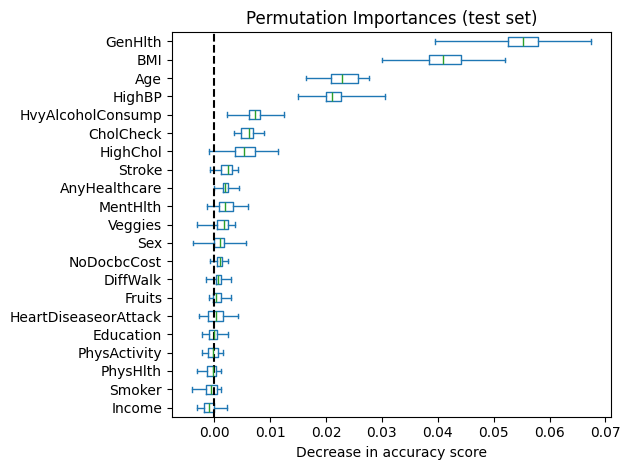
\includegraphics[width=0.75\linewidth]{rysunki/diabetes/pfi_dnn_diabetes.png}
    \caption{Wykres pudełkowy pokazujący wpływ cech na predykcję uzyskany po użyciu metody PFI przy modelu sieci neuronowej dla zbioru dotyczącego diabetyków [źródło własne]}
    \label{fig:pfi_dnn_diabetes}
\end{figure}

\subsubsection{Podsumowanie}
Co zaskakujące, największe ROC AUC osiągnęła niezbyt złożona sieć neuronowa o zaledwie dwóch warstwach ukrytych składających się z 64 neuronów każda. XGBoost Radził sobie najlepiej ze wszystkich z klasyfikacją wariantu '1'. Najgorszą predykcję przedstawiła już wspomniana DNN z wynikiem 80\%, przy czym równie słabo odnajdywała osoby chore na cukrzycę (choć odstępstwo to było niewielkie). Las losowy miał wyniki pośrednie pomiędzy jego konkurentami, nie wyróżnił się w przeciwieństwie do nich niczym szczególnym. 

\begin{table}[H]
\centering
\caption{3 najistotniejsze cechy wskazane przez metody dla każdego z modeli w zbiorze dotyczącym diabetyków}
\label{tab:3_top_diabetes}
\begin{tabular}{|c|c|c|}
\hline
Model & Metoda & 3 najistotniejsze cechy \\ \hline
\multirow{3}{*}{Random Forest}& LIME& HvyAlcoholConsump, GenHlth, Age\\ \cline{2-3} 
 & SHAP& GenHlth, HighBP, BMI\\ \cline{2-3} 
 & PFI& GenHlth, BMI, HighBP\\ \hline
\multirow{3}{*}{XGBoost}& LIME& HighBP, Income, BMI\\ \cline{2-3} & SHAP& GenHlth, BMI, Age\\ \cline{2-3} 
 & PFI& BMI, Age, GenHlth\\ \hline
\multirow{3}{*}{Sieć neuronowa}& LIME& HvyAlcoholConsump, GenHlth, BMI\\ \cline{2-3} & SHAP& GenHlth, BMI, HighBP\\ \cline{2-3} & PFI& GenHlth, BMI, Age\\ \hline
\end{tabular}
\end{table}

Spoglądając na Tabelę \ref{tab:3_top_diabetes} zauważamy, że pojawiły się dwie cechy wśród 3 najistotniejszych występujące w 8 na 9 przypadków. Pierwszą z nich było ,,GenHlth'', które nie wystąpiło tylko w tłumaczeniu LIME modelu XGBoost, gdzie znalazło się na 4 miejscu. Na równi z nią widnieje ,,BMI'', którego zabrakło w wyjaśnieniu LIME dla lasu losowego. Najbardziej nieoczekiwaną zmienną w tym zestawieniu jest ,,Income'' wskazane przez LIME modelu XGBoost. Zdawałoby się, że w zestawieniu jest parę innych, bardziej logicznych do uznania cech, takich jak ,,Age'' czy ,,HvyAlcoholConsump'' pojawiające się w innych wytłumaczeniach. 
Niezwykle wiele danych zostało odrzuconych przez metodę PFI sieci neuronowej, w jej tłumaczeniu znalazło się tylko 6 zmiennych z 21. Analizując cechy najmniej wpływowe dostrzegamy, że często powtarzają się wśród nich: ,,AnyHealthcare'', ,,Veggies'', ,,Fruits'' oraz ,,CholCheck''. Chociaż w niektórych zestawieniach pojawiają się wysoko na liście.


\subsection{UCI Heart Disease Data}
\subsubsection{Random Forest}
\begin{table}[H]
 \centering
    \caption{Wyniki uzyskane przy modelu Random Forest dla zbioru dotyczącego choroby serca}
\begin{tabular}{|ccccc|}
\hline
\multicolumn{5}{|c|}{ROC AUC: 0.85}                                                                                                                       \\ \hline
\multicolumn{1}{|c|}{Klasa \textbackslash Metryka} & \multicolumn{1}{c|}{Precyzja} & \multicolumn{1}{c|}{Czułość} & \multicolumn{1}{c|}{F1-score} & Liczba \\ \hline
\multicolumn{1}{|c|}{0}                            & \multicolumn{1}{c|}{0.80}     & \multicolumn{1}{c|}{0.83}    & \multicolumn{1}{c|}{0.81}     & 82    \\ \hline
\multicolumn{1}{|c|}{1}                            & \multicolumn{1}{c|}{0.54}     & \multicolumn{1}{c|}{0.64}    & \multicolumn{1}{c|}{0.59}     & 53    \\ \hline
\multicolumn{1}{|c|}{2}                            & \multicolumn{1}{c|}{0.30}     & \multicolumn{1}{c|}{0.27}    & \multicolumn{1}{c|}{0.29}     & 22    \\ \hline
\multicolumn{1}{|c|}{3}                            & \multicolumn{1}{c|}{0.40}     & \multicolumn{1}{c|}{0.29}    & \multicolumn{1}{c|}{0.33}     & 21    \\ \hline
\multicolumn{1}{|c|}{4}                            & \multicolumn{1}{c|}{1.00}     & \multicolumn{1}{c|}{0.17}    & \multicolumn{1}{c|}{0.29}     & 6     \\ \hline
\multicolumn{5}{|c|}{}                                                                                                                                    \\ \hline
\multicolumn{1}{|c|}{Dokładność}                   & \multicolumn{3}{c|}{0.62}                                                                    & 184   \\ \hline
\multicolumn{1}{|c|}{Śr. arytmetyczna}                    & \multicolumn{1}{c|}{0.61}     & \multicolumn{1}{c|}{0.44}    & \multicolumn{1}{c|}{0.46}     & 184   \\ \hline
\multicolumn{1}{|c|}{Śr. ważona}                   & \multicolumn{1}{c|}{0.63}     & \multicolumn{1}{c|}{0.62}    & \multicolumn{1}{c|}{0.61}     & 184   \\ \hline
\end{tabular}
    \label{tab:heart_disease_random_forest_metrics}
\end{table}

Poprzez analizę wyników uzyskanych przez las losowy zamieszczonych w Tabela \ref{tab:heart_disease_random_forest_metrics} zauważamy, że  wykazał on dokładność na poziomie 62\%. Wyniki średniej arytmetycznej osiągnęły dla precyzji 61\%, czułości 44\%, a F1-score 46\%. Z kolei średnia ważona uzyskała wartości kolejno: 63\%, 62\% oraz 61\%. W macierzy pomyłek pokazanej na Rys. \ref{fig:confusion_matrix_random_forest_heart_disease} dostrzegamy, że model tylko raz i to poprawnie zakwalifikował 1 z próbek do '4' kategorii. Z drugiej strony bardzo dobrze radził sobie przy poprawnej ocenie rekordów należących do dwóch pierwszych wariantów. Z 82 osobników klasy '0' właściwie rozpoznał 68. Daje to precyzję na poziomie 80\%. Czułość wyniosła 83\%, co przyczynia się do F1-score z wartością 81\%. Pole powierzchni pod krzywą ROC wyniosło w przybliżeniu 0.85.

\begin{figure}[H]
    \centering
    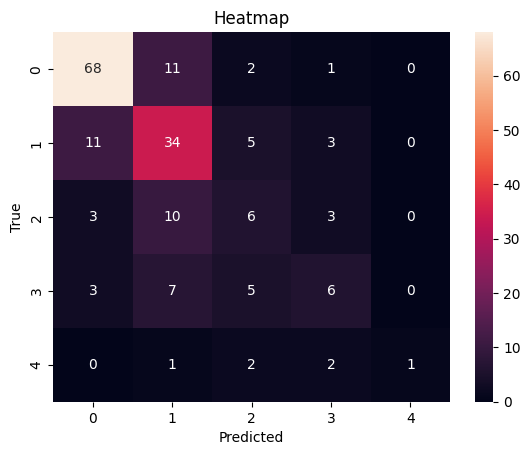
\includegraphics[width=0.75\linewidth]{rysunki/heart/macierz_pomylek_rf_heart.png}
    \caption{Macierz pomyłek modelu Random Forest dla zbioru dotyczącego choroby serca [źródło własne]}
    \label{fig:confusion_matrix_random_forest_heart_disease}
\end{figure}

Wykres zaprezentowany na Rys. \ref{fig:lime_barchar_rf_heart} pokazuje, że według metody \textbf{LIME} najważniejszą informację predykcyjną w wariancie '0' i '1' zawiera ,,exang'', z czego w pierwszym przypadku jej waga wynosi ok. 0.175, a drugim - 0.125. ,,dataset'' było czynnikiem przeważającym nad klasyfikacją do '2' i '3' kategorii, a ,,oldpeak'' - '4'. Cechą wnoszącą najmniej okazało się być ,,sex'', której średnia wag wyniosła 0 dla każdej z klas.

\begin{figure}[H]
    \centering
    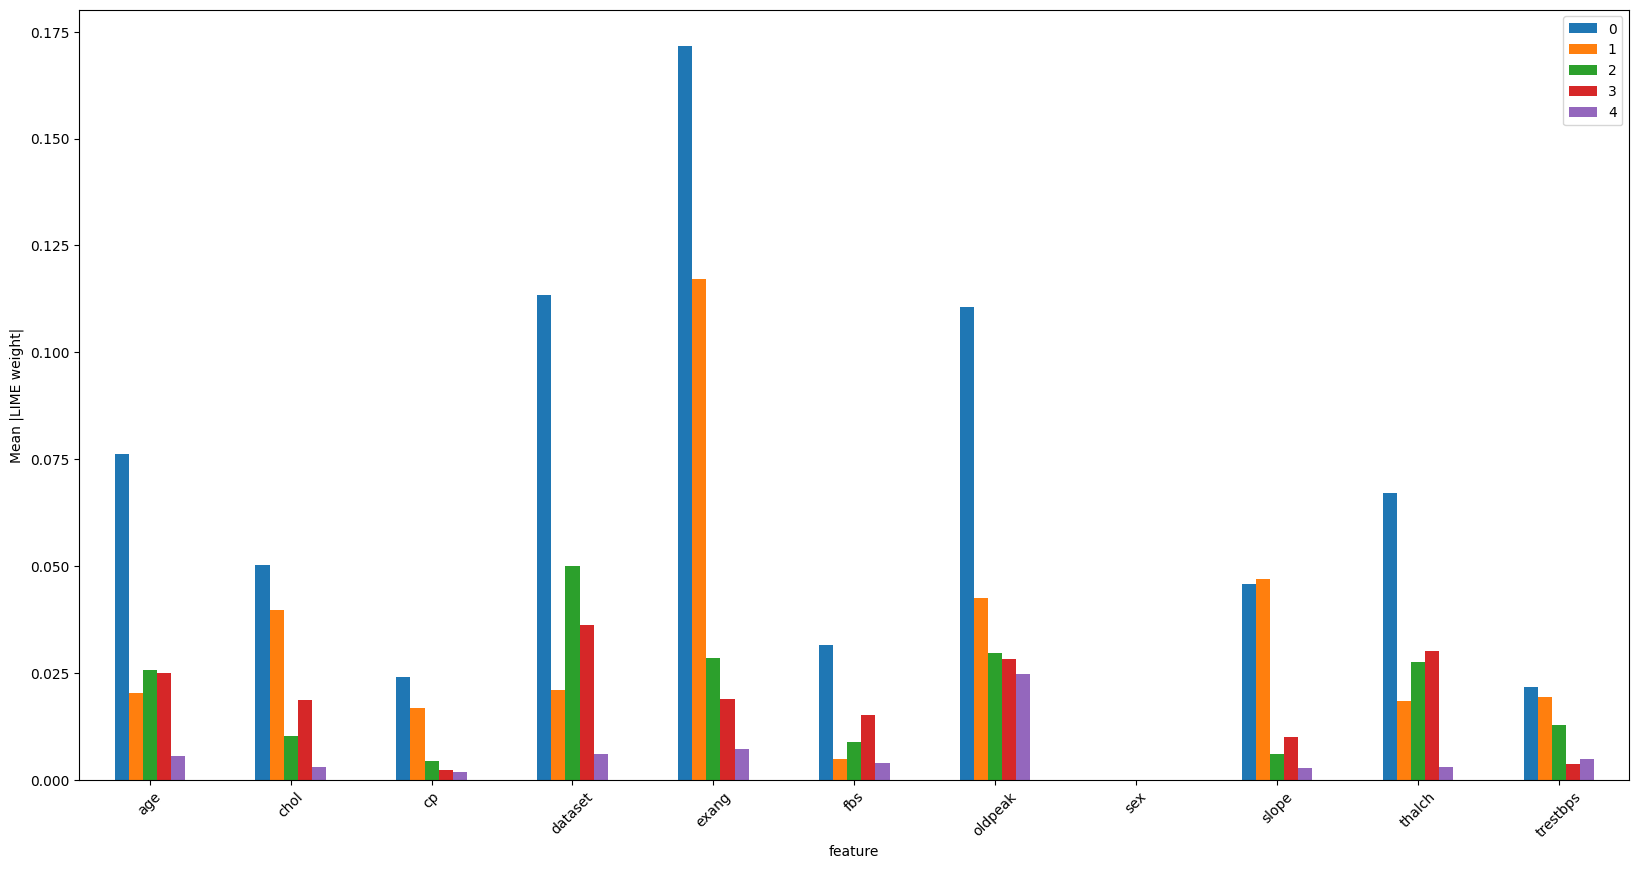
\includegraphics[width=0.9\linewidth]{rysunki/heart/lime_barchar_rf_heart.png}
    \caption{Wykres słupkowy średnich wartości bezwzględnych wag LIME dla każdej z klasy modelu Random Forest zbioru dotyczącego choroby serca [źródło własne]}
    \label{fig:lime_barchar_rf_heart}
\end{figure}

Z Rys. \ref{fig:lime_absolutemeanplot_rf_heart} można wyczytać, że najważniejszą cechą jest ,,exang'' osiągająca wagę 0.07. Jak zostało to wskazane na poprzedniej wizualizacji, dawała ona najwięcej wartości predykcyjnej dla klas '0' i '1'. Spadek,,oldpeak'' zajął drugie miejsce pod względem danego porównania z wartością prawie 0.05. Zaraz po nim znajduje się ,,dataset'' z lekko mniejszą miarą na poziomie ok. 0.045. Wagę 0 osiągnęła cecha ,,sex''. Trochę więcej do predykcji wnosiło ,,cp'' z wartością 0.01 oraz ,,trestbps'' z 0.0125.

\begin{figure}[H]
    \centering
    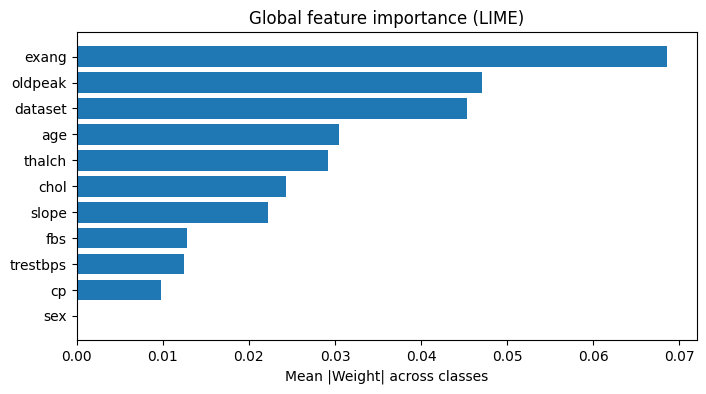
\includegraphics[width=0.75\linewidth]{rysunki/heart/lime_absolutemeanplot_rf_heart.png}
    \caption{Wykres średnich obliczonych z bezwzględnych wartości wag LIME modelu Random Forest zbioru dotyczącego choroby serca [źródło własne]}
    \label{fig:lime_absolutemeanplot_rf_heart}
\end{figure}

Z wykresu opisującego wyniki metody \textbf{SHAP}, znajdującego się na Rys. \ref{fig:shap_barchar_rf_heart}, możemy zauważyć, że najbardziej odznaczającym się słupkiem jest ten, odpowiadający ,,cp'', które osiąga dla wariantu '0' wartość równą w przybliżeniu 0.13. Podobnie jest w przypadku '1' stopnia, gdzie cecha ta wynosi ok. 0.065. Dla kategorii '2' i '3' najważniejszym wyznacznikiem jest ,,dataset'', a '4' - ,,oldpeak''. Z wykresu wynika, że najmniej istotną informację wnosi ,,fbs''.

\begin{figure}[H]
    \centering
    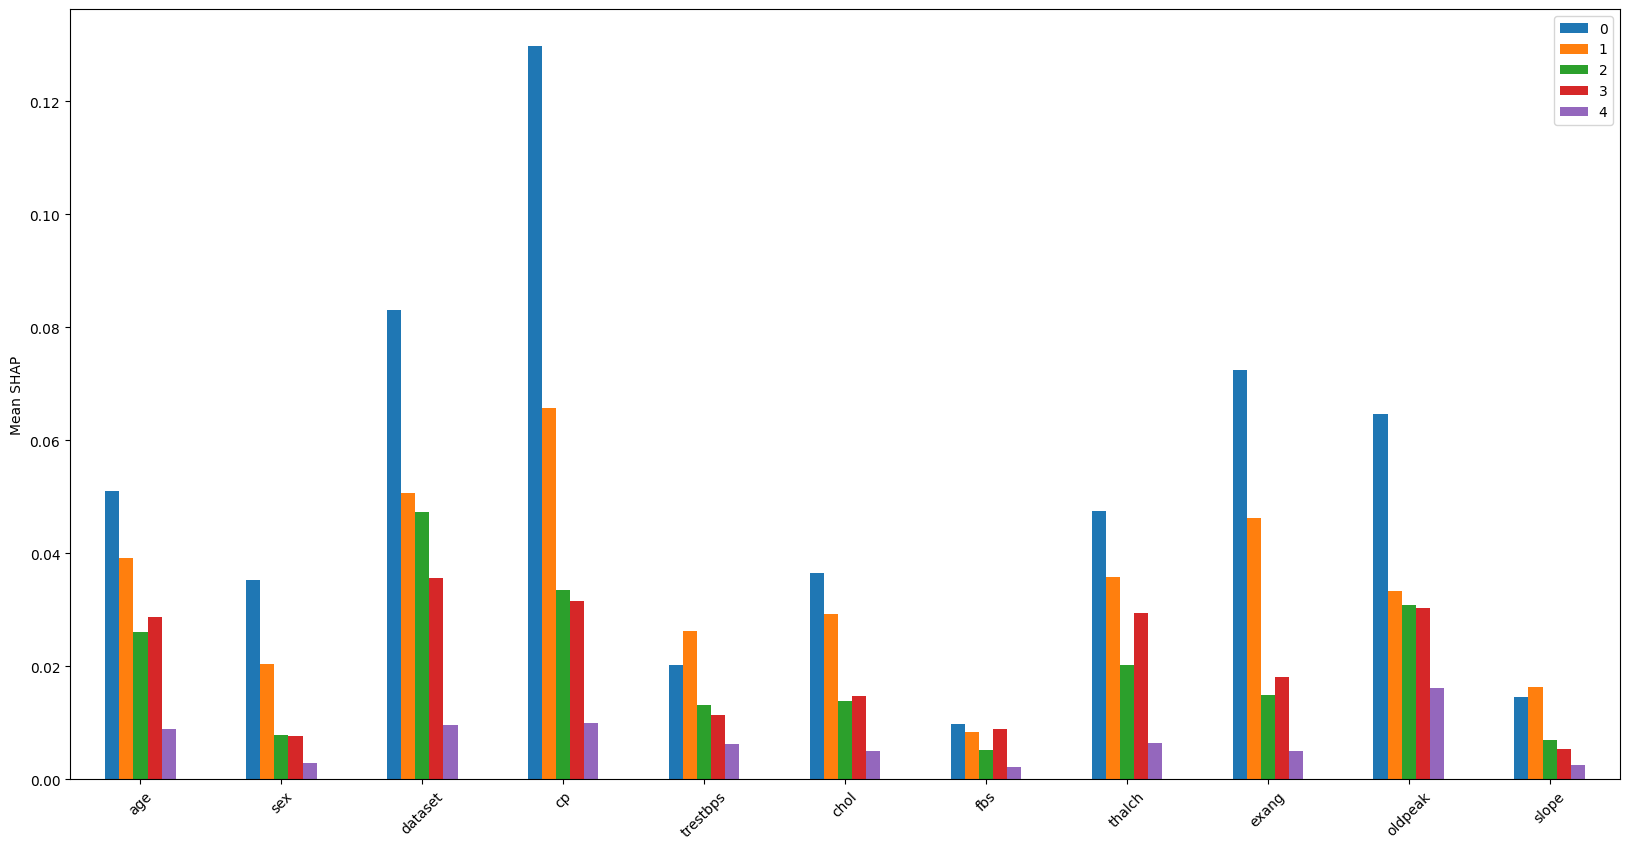
\includegraphics[width=0.9\linewidth]{rysunki/heart/shap_barchar_rf_heart.png}
    \caption{Wykres słupkowy średnich wartości SHAP dla każdej z klasy modelu Random Forest zbioru dotyczącego choroby serca [źródło własne]}
    \label{fig:shap_barchar_rf_heart}
\end{figure}

Na wykresie zwizualizowanym na Rys. \ref{fig:shap_absolutemeanplot_rf_heart} również zauważamy, że największą istotność posiada ,,cp'' oraz ,,dataset''. Na kolejnych miejscach znajdują się ,,oldpeak'' oraz ,,age''. Są to głównie kolumny wskazane podczas badań wpływu cech z podziałem na klasy. Tutaj również zmiennymi posiadającymi znikomy wpływ okazały się być ,,slope'' i ,,fbs''. 

\begin{figure}[H]
    \centering
    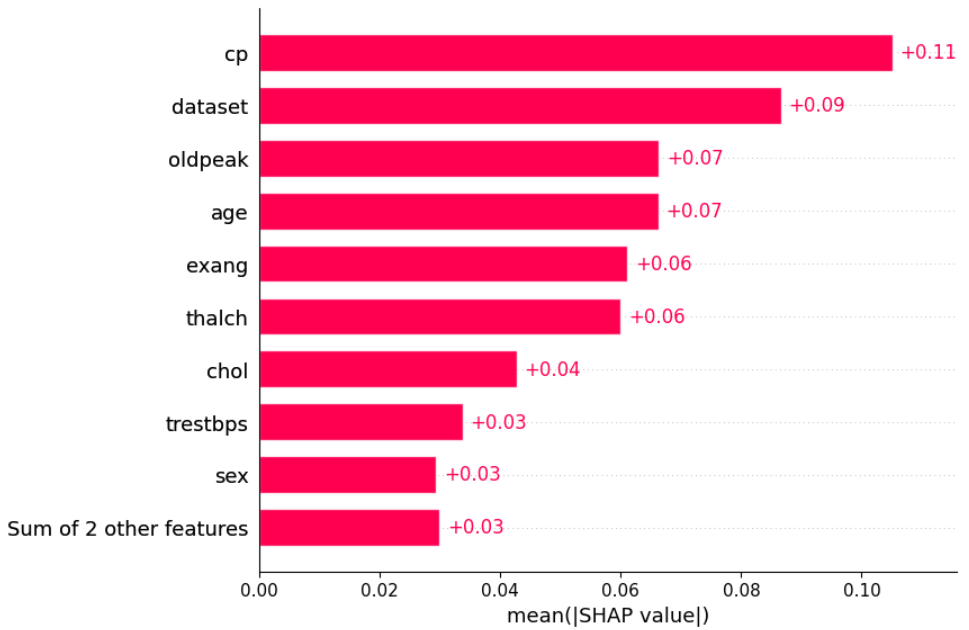
\includegraphics[width=0.75\linewidth]{rysunki/heart/shap_absolutemeanplot_rf_heart.png}
    \caption{Wykres średnich obliczonych z bezwzględnych wartości SHAP modelu Random Forest zbioru dotyczącego choroby serca [źródło własne]}
    \label{fig:shap_absolutemeanplot_rf_heart}
\end{figure}

\iffalse
Z zamieszczonego na Rys. \ref{fig:shap_beeswarm_rf_heart} wykresu można zauważyć najbardziej widoczne zależności m.in. dla ,,cp'', gdzie istnieją dwa skupiska niebieskich kropek. Oznaczają one, że dla jednej z klas predykcyjnych brak bólu klatki piersiowej znacznie zmiejsza prawdopodobieństwo przypisania do tej klasy, a dla drugiej - trochę je zwiększa. Z kolei wysokie liczby świadczą o braku bądź pozytywnym znaczeniu, a średnie w głównej mierze podwyższają predykcję. Kolejną kolumną wartą uwagi jest ,,sex'' osiągająca wartości SHAP oscylujące wokół 0 kiedy sama jest wysoka, natomiast pozytywny wpływ o ile jest mała. Odwrotna sytuacja odbywa się w przypadku ,,exang'', gdzie środkowa część składa się w głównej mierze z niebieskich kropek, a brzegi z czerwonych. W wielu obszarach punkty są przemieszane nie oferując zbyt wiele przydatnych informacji na temat przewidywań. Do takich miejsc możemy zaliczyć środkowe części dla cech ,,thalch'', ,,chol'', czy ,,trestbps''.

\begin{figure}[H]
    \centering
    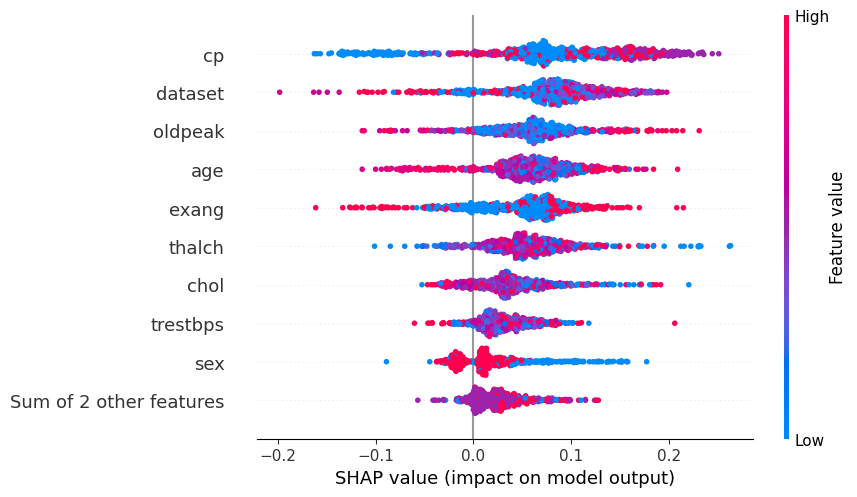
\includegraphics[width=1\linewidth]{rysunki/heart/shap_beeswarm_rf_heart.png}
    \caption{Wykres typu ,,beeswarm'' wartości SHAP modelu Random Forest zbioru dotyczącego choroby serca [źródło własne]}
    \label{fig:shap_beeswarm_rf_heart}
\end{figure}
\fi

\begin{xltabular}{\textwidth}{|c|c|c|}
    \caption{Wyniki uzyskane po użyciu metody PFI przy modelu Random Forest dla zboru dotyczącego choroby serca}
    \label{tab:heart_disease_random_forest_pfi}\\ \hline
    Cecha & Średnia & Odchylenie standardowe \\ \hline
    \endfirsthead
        dataset & 0.175 &  0.012 \\ \hline
        cp & 0.175 &  0.012 \\ \hline
        age & 0.128 &  0.011 \\ \hline
        oldpeak & 0.116 &  0.010 \\ \hline
        thalch & 0.090 &  0.007 \\ \hline
        chol & 0.071 &  0.006 \\ \hline
        exang & 0.069 &  0.006 \\ \hline
        trestbps & 0.049 &  0.005 \\ \hline
        sex & 0.026 &  0.005 \\ \hline
        fbs & 0.015 &  0.002 \\ \hline
        slope & 0.005 &  0.002 \\ \hline
\end{xltabular}

Według metody \textbf{PFI}, jak wynika z Tabela \ref{tab:heart_disease_random_forest_pfi} oraz Rys. \ref{fig:box_plot_rf_pfi} wszystkie kolumny okazały się być ważne w zadaniu klasyfikacji próbek. Najważniejszą cechą okazało się być ,,dataset'', której średnia istotność wyniosła 17,5\% z odchyleniem standardowym wynoszącym 0,012. Na drugim miejscu plasuje się ,,cp'' również ze średnią 17,5\%, a trzecim - ,,age'' z wynikiem 12,8\%. Najmniej znaczącą informację niósł za sobą ,,slope'', bo zaledwie 0.5\% z rozbieżnościami na poziomie 0.002. 

\begin{figure}[H]
    \centering
    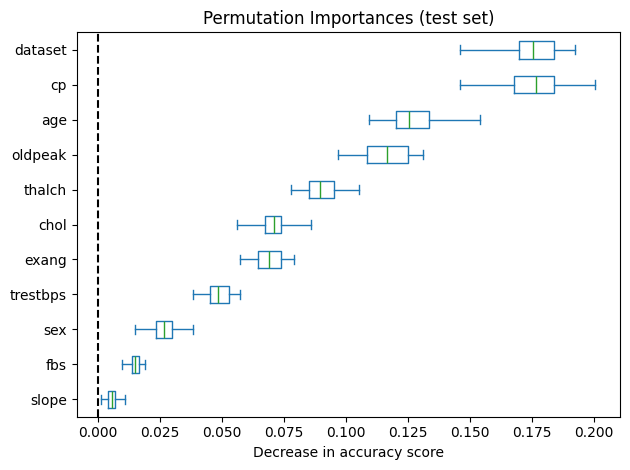
\includegraphics[width=0.75\linewidth]{rysunki/heart/pfi_rf_heart.png}
    \caption{Wykres pudełkowy pokazujący wpływ cech na predykcję uzyskany po użyciu metody PFI przy modelu Random Forest dla zbioru dotyczącego choroby serca [źródło własne]}
    \label{fig:box_plot_rf_pfi}
\end{figure}

\subsubsection{XGBoost}
\begin{table}[H]
    \centering
    \caption{Wyniki uzyskane przy modelu XGBoost dla zbioru dotyczącego choroby serca}
\begin{tabular}{|ccccc|}
\hline
\multicolumn{5}{|c|}{ROC AUC: 0.84}                                                                                                                       \\ \hline
\multicolumn{1}{|c|}{Klasa \textbackslash Metryka} & \multicolumn{1}{c|}{Precyzja} & \multicolumn{1}{c|}{Czułość} & \multicolumn{1}{c|}{F1-score} & Liczba \\ \hline
\multicolumn{1}{|c|}{0}                            & \multicolumn{1}{c|}{0.80}     & \multicolumn{1}{c|}{0.82}    & \multicolumn{1}{c|}{0.81}     & 82    \\ \hline
\multicolumn{1}{|c|}{1}                            & \multicolumn{1}{c|}{0.56}     & \multicolumn{1}{c|}{0.62}    & \multicolumn{1}{c|}{0.59}     & 53    \\ \hline
\multicolumn{1}{|c|}{2}                            & \multicolumn{1}{c|}{0.37}     & \multicolumn{1}{c|}{0.32}    & \multicolumn{1}{c|}{0.34}     & 22    \\ \hline
\multicolumn{1}{|c|}{3}                            & \multicolumn{1}{c|}{0.43}     & \multicolumn{1}{c|}{0.43}    & \multicolumn{1}{c|}{0.43}     & 21    \\ \hline
\multicolumn{1}{|c|}{4}                            & \multicolumn{1}{c|}{1.00}     & \multicolumn{1}{c|}{0.17}    & \multicolumn{1}{c|}{0.29}     & 6     \\ \hline
\multicolumn{5}{|c|}{}                                                                                                                                    \\ \hline
\multicolumn{1}{|c|}{Dokładność}                   & \multicolumn{3}{c|}{0.64}                                                                    & 184   \\ \hline
\multicolumn{1}{|c|}{Śr. arytmetyczna}                    & \multicolumn{1}{c|}{0.63}     & \multicolumn{1}{c|}{0.47}    & \multicolumn{1}{c|}{0.49}     & 184   \\ \hline
\multicolumn{1}{|c|}{Śr. ważona}                   & \multicolumn{1}{c|}{0.64}     & \multicolumn{1}{c|}{0.64}    & \multicolumn{1}{c|}{0.63}     & 184   \\ \hline
\end{tabular}
    \label{tab:heart_disease_xgboost_metrics}
\end{table}

XGBoost uczony i sprawdzany na tych samych danych (zbiorze treningowym i testowym), jak wskazuje Tabela \ref{tab:heart_disease_xgboost_metrics} osiągnął wynik dokładności wynoszący 64\%. Jego średnie arytmetyczne uzyskały: dla precyzji 63\%, czułości 47\%, a F1-score 49\%. Ważone były wyższe i wskazały w tej samej kolejności: 64\%, 64\% i 63\%. Miara ROC AUC tutaj wyniosła 0.84. XGBoost zakwalifikował tylko jeden z przypadków do klasy '4', który rzeczywiście do niej należał. Dobrze radził sobie z obiektami kategorii '0', '1' i potencjalnie '3'. Analiza Rys. \ref{fig:confusion_matrix_xgboost_heart_disease} sugeruje, że w miarę często zdarza mu się pomylić przypadki należące do stadium '0' i '1', a lepiej idzie mu odnajdywanie próbek zaklasyfikowanych jako '3' niż '2' pomimo zbliżonej wielkości grup.

\begin{figure}[H]
    \centering
    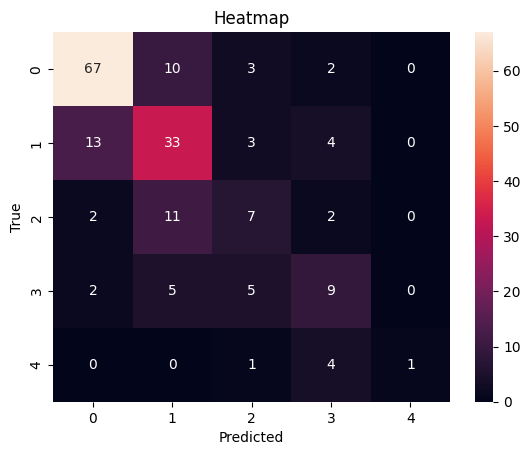
\includegraphics[width=0.75\linewidth]{rysunki/heart/macierz_pomylek_xgb_heart.png}
    \caption{Macierz pomyłek modelu XGBoost dla zbioru dotyczącego choroby serca [źródło własne]}
    \label{fig:confusion_matrix_xgboost_heart_disease}
\end{figure}

Na wykresie znajdującym się na Rys. \ref{fig:lime_barchar_xgb_heart} zaprezentowane zostały wyniki metody \textbf{LIME}. Najbardziej odznaczającą się cechą ,,exang'', która ma największą istotność dla klasy '0', gdzie waga jej wynosi ponad 0.21 i '1', dla której zbliża się ona do 0.2. W przypadku '2' najważniejszą wartość wnosi ,,dataset'', a '3' i '4' ,,oldpeak''. Najmniej istotna okazała się być kolumna ,,sex'' z wagą 0.  

\begin{figure}[H]
    \centering
    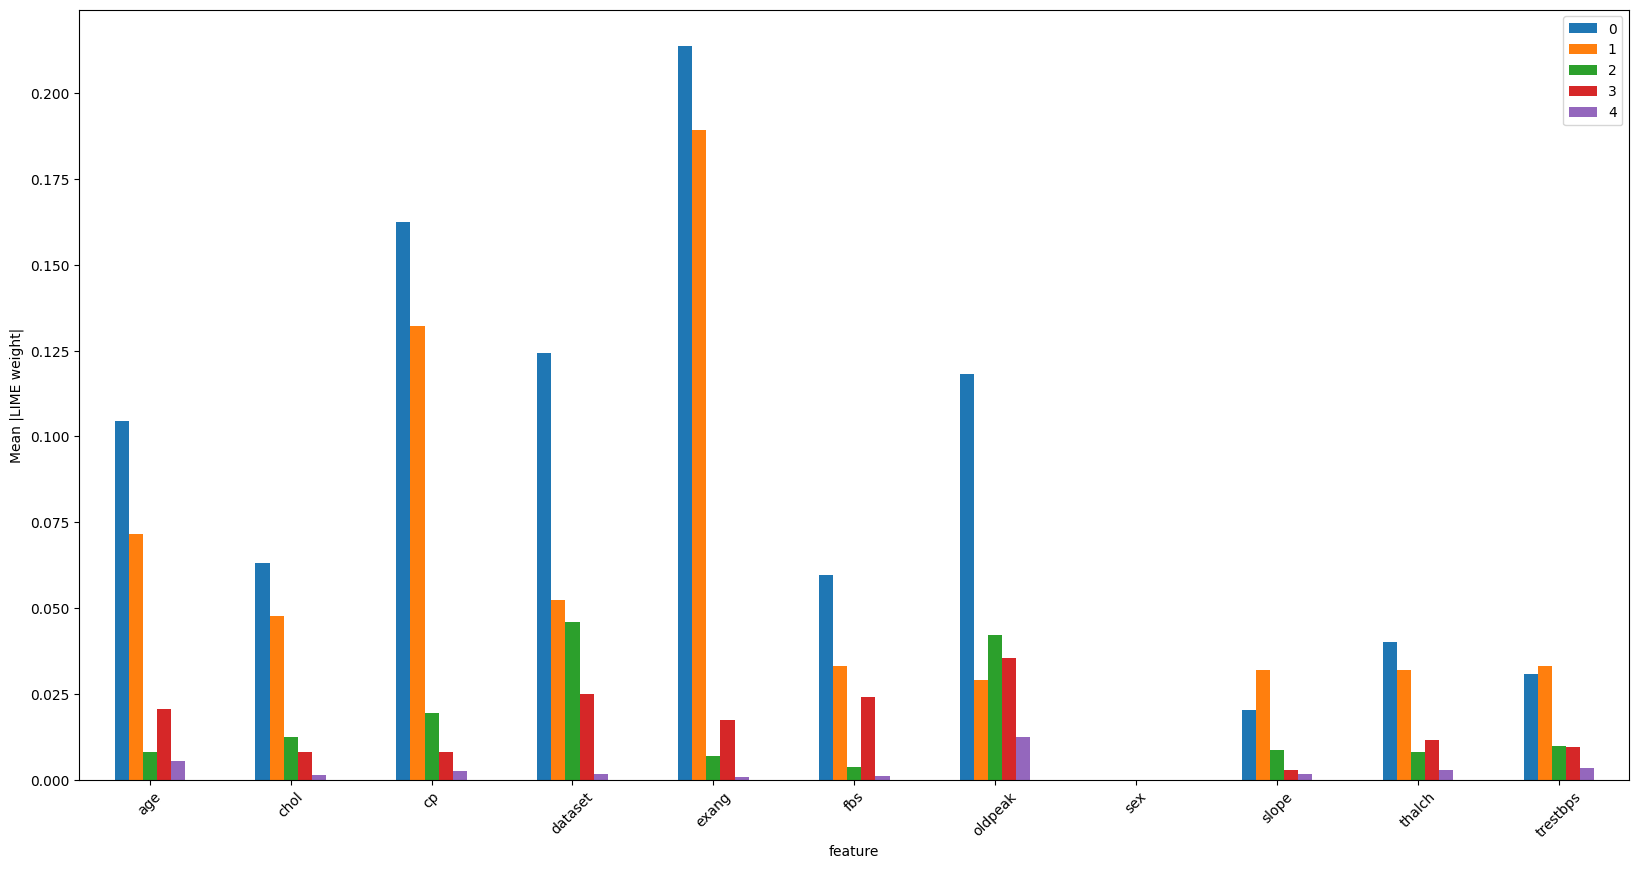
\includegraphics[width=0.9\linewidth]{rysunki/heart/lime_barchar_xgb_heart.png}
    \caption{Wykres słupkowy średnich wartości bezwzględnych wag LIME dla każdej z klasy modelu XGBoost zbioru dotyczącego choroby serca [źródło własne]}
    \label{fig:lime_barchar_xgb_heart}
\end{figure}

Wykres zaprezentowany na Rys. \ref{fig:lime_absolutemeanplot_xgb_heart} potwierdza znaczący wpływ cechy odpowiadającej za ,,exang'' i ustala jej wagę na ok. 0.085. Kolejną wskazaną przez niego wysoce istotną zmienną jest ,,cp'', a następnie ,,dataset''. Tak samo jak na poprzedniej wizualizacji ,,sex'' nie ma jakiegokolwiek znaczenia i jego waga wynosi 0. Z również dosyć nikłymi wynikami plasują się: ,,thalch'', spoczynkowe,,trestbps'' oraz ,,slope''; a ich wartości nie przekraczają 0.02. 

\begin{figure}[H]
    \centering
    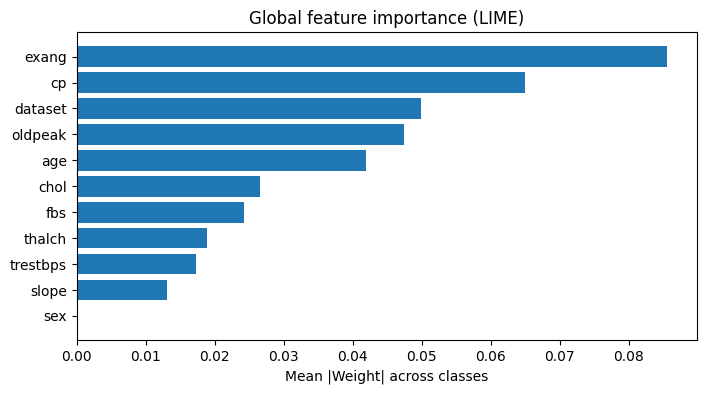
\includegraphics[width=0.75\linewidth]{rysunki/heart/lime_absolutemeanplot_xgb_heart.png}
    \caption{Wykres średnich obliczonych z bezwzględnych wartości wag LIME modelu XGBoost zbioru dotyczącego choroby serca [źródło własne]}
    \label{fig:lime_absolutemeanplot_xgb_heart}
\end{figure}

Według metody \textbf{SHAP} najbardziej odznaczającą się jest ,,oldpeak'' klasy '4' osiągający wartość ok. 1.15, co zauważamy z wykresu przedstawionego na Rys. \ref{fig:shap_barchar_xgb_heart}. Drugą miarą pod względem wielkości otrzymanego wyniku jest ta wskazująca na ,,dataset'' wariantu '2' i wynosi ona 0.85. Zbliżoną liczbę uzyskało ,,cp'' dla przypadku '0', bo mniejszą zaledwie o 0.05. Następną pod względem wielkości kolumnę posiada ,,thalch'' klasy '3' z wartością ok 0.7. Na '1' największy wpływ ma ,,chol'', którego istotność osiągnęła w przybliżeniu 0.45. Najmniej znaczącą cechą w większości diagnoz wydaje się być ,,fbs''.    

\begin{figure}[H]
    \centering
    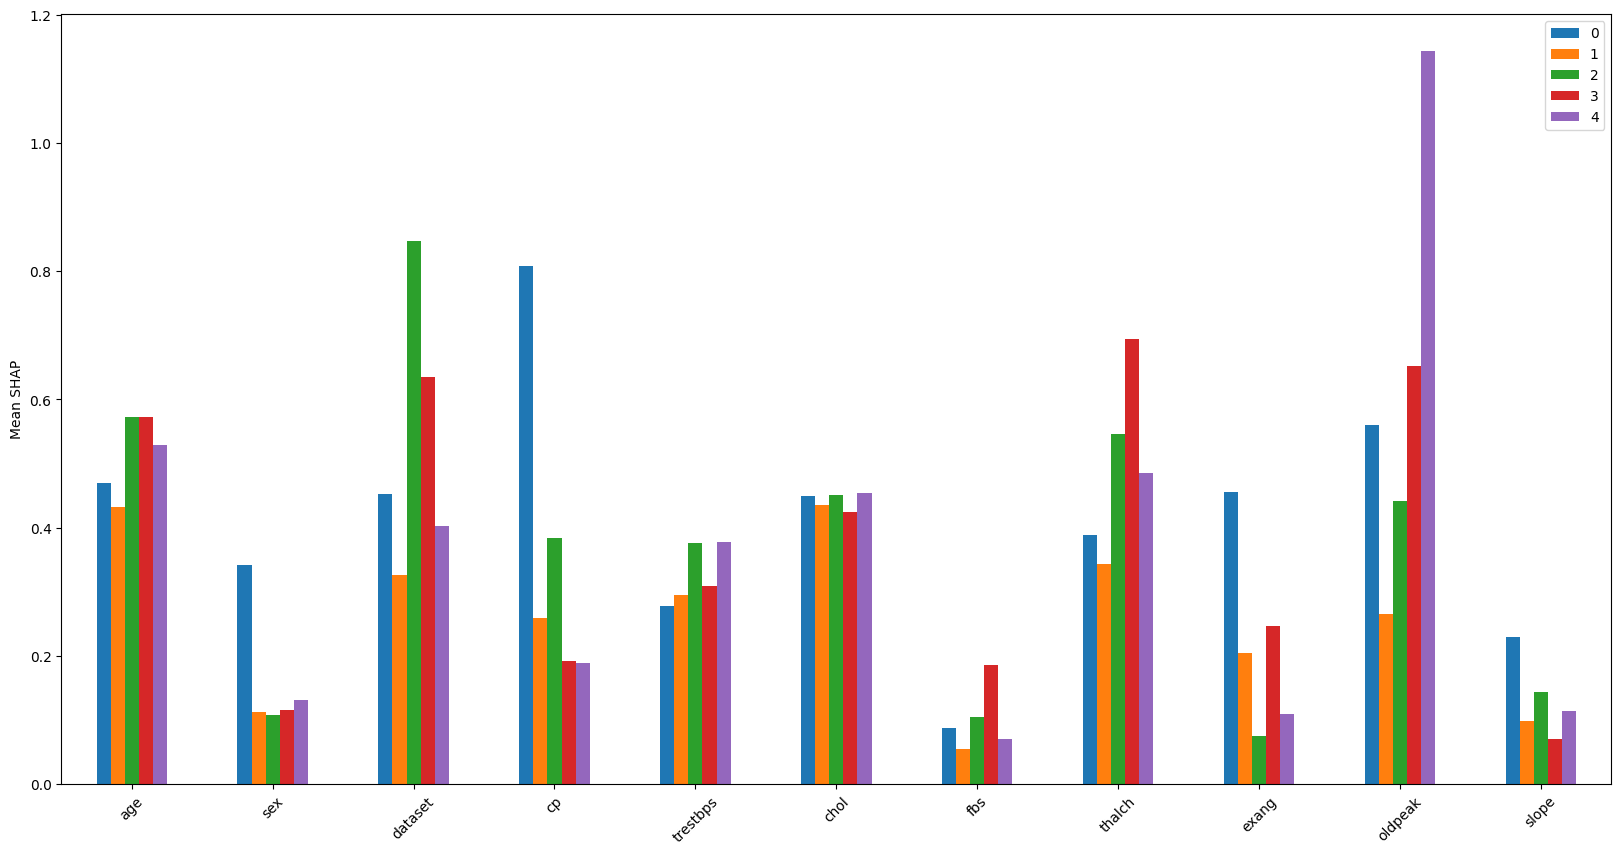
\includegraphics[width=0.9\linewidth]{rysunki/heart/shap_barchar_xgb_heart.png}
    \caption{Wykres słupkowy średnich wartości SHAP dla każdej z klasy modelu XGBoost zbioru dotyczącego choroby serca [źródło własne]}
    \label{fig:shap_barchar_xgb_heart}
\end{figure}

Z wizualizacji na Rys. \ref{fig:shap_absolutemeanplot_xgb_heart} możemy wyczytać, że za najistotniejsze elementy metoda uznała na równi ,,age'' i ,,cp'', którym obu przyporządkowała wartość 0.54. Kolejną również parą niosącą za sobą najważniejsze informacje jest ,,thalch'' oraz ,,oldpeak'' z miarami 0.45. Najmniej wartościowe okazało się być ,,slope'', a także ,,fbs'', które zostały zaprezentowane w słupku oznaczonym jako suma.

\begin{figure}[H]
    \centering
    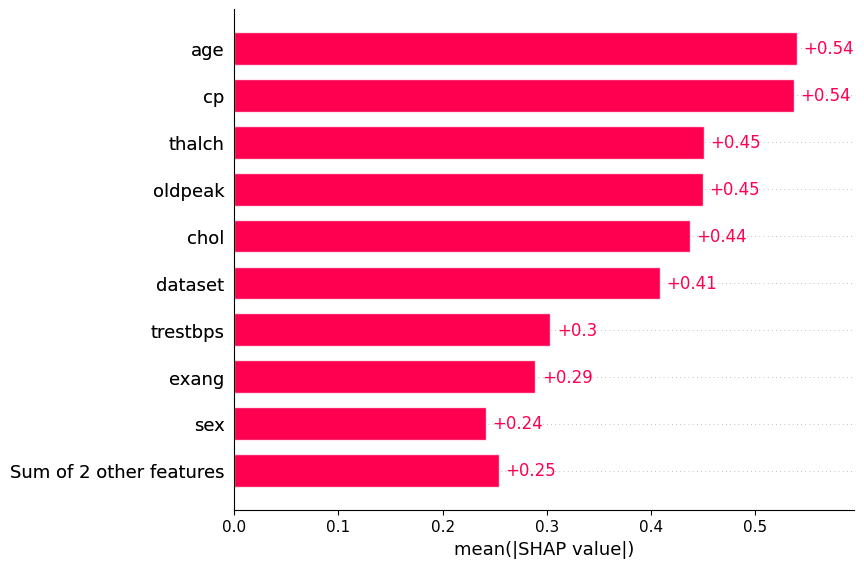
\includegraphics[width=0.75\linewidth]{rysunki/heart/shap_absolutemeanplot_xgb_heart.png}
    \caption{Wykres średnich obliczonych z bezwzględnych wartości SHAP modelu XGBoost zbioru dotyczącego choroby serca [źródło własne]}
    \label{fig:shap_absolutemeanplot_xgb_heart}
\end{figure}

\iffalse
Z wykresu ,,rój pszczół'' znajdującym się na Rys. \ref{fig:shap_beeswarm_xgb_heart} ciężko dla większości cech wysnuć jakieś istotne wnioski. Wiele miejsc przeplata się kolorystycznie nie oferując zbytniego wglądu w rozkład wartości w zależności od ich istotności. Jedną z nielicznych zmiennych pozwalających na trafne obserwacje jest ,,cp'', której małe miary mają negatywny bądź znikomy wpływ na predykcję, wysokie lekko ujemny oraz dodatni, a średnie duży dodatni przekaz. Kolejną taką cechą może być ,,exang''', której małe wartości oscylują wokół 0, ale z kolei duże już są rozłożone po całości zajmowanego obszaru. W przypadku ,,sex'' sprawa jest odwrotna - duże wartości mieszczą się w pobliżu 0, natomiast małe zajmują głównie prawą, dodatnią stronę osi. 

\begin{figure}[H]
    \centering
    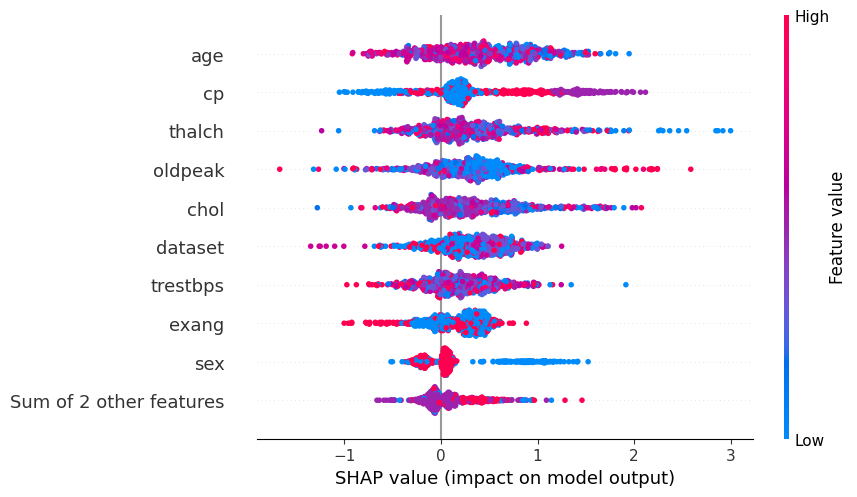
\includegraphics[width=1\linewidth]{rysunki/heart/shap_beeswarm_xgb_heart.png}
    \caption{Wykres typu ,,beeswarm'' wartości SHAP modelu XGBoost zbioru dotyczącego choroby serca [źródło własne]}
    \label{fig:shap_beeswarm_xgb_heart}
\end{figure}
\fi

\begin{xltabular}{\textwidth}{|c|c|c|}
    \caption{Wyniki uzyskane po użyciu metody PFI przy modelu XGBoost dla zbioru dotyczącego choroby serca}
    \label{tab:heart_disease_xgb_pfi}\\ \hline
    Cecha & Średnia & Odchylenie standardowe \\ \hline
    \endfirsthead
        age     & 0.150 &  0.012 \\ \hline
        oldpeak & 0.127 &  0.010 \\ \hline
        chol    & 0.126 &  0.011 \\ \hline
        thalch  & 0.121 &  0.008 \\ \hline
        dataset & 0.098 &  0.009 \\ \hline
        trestbps& 0.072 &  0.006 \\ \hline
        cp      & 0.063 &  0.006 \\ \hline
        exang   & 0.013 &  0.003 \\ \hline
        sex     & 0.013 &  0.003 \\ \hline
        fbs     & 0.006 &  0.002 \\ \hline
        slope   & 0.005 &  0.001 \\ \hline
\end{xltabular}

\textbf{PFI} uznał wszystkie cechy za istotne w przewidywaniu. Jak wskazuje Tabela \ref{tab:heart_disease_xgb_pfi} najważniejszą informację niósł za sobą ,,age'', przez którego permutację model stracił na dokładności całe 15\% z odchyleniem standardowym rzędu  0.012. Kolejnymi najbardziej znaczącymi kolumnami okazały się być - ,,oldpeak'' z istotnością 12.7\% oraz cholesterol,,chol'' z 12.6\%. Najniżej w tym rankingu możemy zauważyć ,,slope'', który osiągnął średnią istotność na poziomie jedynie 0.5\%. 

\begin{figure}[H]
    \centering
    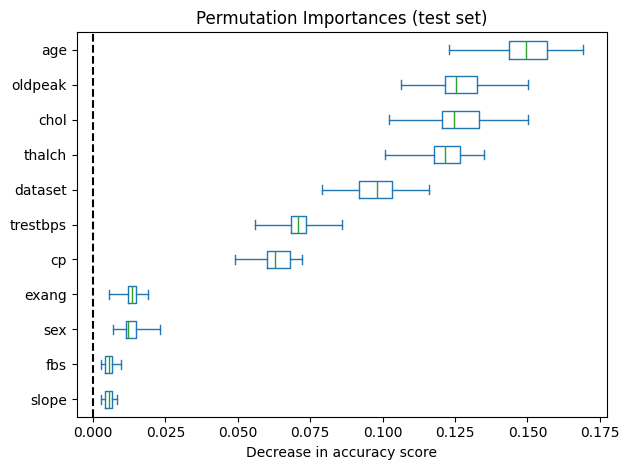
\includegraphics[width=0.75\linewidth]{rysunki/heart/pfi_xgb_heart.png}
    \caption{Wykres pudełkowy pokazujący wpływ cech na predykcję uzyskany po użyciu metody PFI przy modelu XGBoost dla zbioru dotyczącego choroby serca [źródło własne]}
    \label{fig:box_plot_xgb_pfi}
\end{figure}

\subsubsection{Sieć neuronowa}
\begin{table}[H]
\centering
    \caption{Wyniki uzyskane przy modelu sieci neuronowej dla zbioru dotyczącego choroby serca}
\begin{tabular}{|ccccc|}
\hline
\multicolumn{5}{|c|}{ROC AUC: 0.80}  \\ \hline
\multicolumn{1}{|c|}{Klasa \textbackslash Metryka} & \multicolumn{1}{c|}{Precyzja} & \multicolumn{1}{c|}{Czułość} & \multicolumn{1}{c|}{F1-score} & Liczba \\ \hline
\multicolumn{1}{|c|}{0}                            & \multicolumn{1}{c|}{0.85}     & \multicolumn{1}{c|}{0.85}    & \multicolumn{1}{c|}{0.85}     & 82    \\ \hline
\multicolumn{1}{|c|}{1}                            & \multicolumn{1}{c|}{0.47}     & \multicolumn{1}{c|}{0.58}    & \multicolumn{1}{c|}{0.52}     & 53    \\ \hline
\multicolumn{1}{|c|}{2}                            & \multicolumn{1}{c|}{0.21}     & \multicolumn{1}{c|}{0.14}    & \multicolumn{1}{c|}{0.17}     & 22    \\ \hline
\multicolumn{1}{|c|}{3}                            & \multicolumn{1}{c|}{0.29}     & \multicolumn{1}{c|}{0.29}    & \multicolumn{1}{c|}{0.29}     & 21    \\ \hline
\multicolumn{1}{|c|}{4}                            & \multicolumn{1}{c|}{0.00}     & \multicolumn{1}{c|}{0.00}    & \multicolumn{1}{c|}{0.00}     & 6     \\ \hline
\multicolumn{5}{|c|}{}  \\ \hline
\multicolumn{1}{|c|}{Dokładność}                   & \multicolumn{3}{c|}{0.60} & 184   \\ \hline
\multicolumn{1}{|c|}{Śr. arytmetyczna}                    & \multicolumn{1}{c|}{0.36}     & \multicolumn{1}{c|}{0.37}    & \multicolumn{1}{c|}{0.37}     & 184   \\ \hline
\multicolumn{1}{|c|}{Śr. ważona}                   & \multicolumn{1}{c|}{0.57}     & \multicolumn{1}{c|}{0.60}    & \multicolumn{1}{c|}{0.58}     & 184   \\ \hline
\end{tabular}
    \label{tab:heart_disease_dnn_metrics}
\end{table}

Za pomocą funkcji GridSearchCV przeszukałam przestrzeń rozwiązań, dzięki czemu spośród wskazanych hiperparametrów uzyskałam odpowiedź, które są najodpowiedniejsze do danego problemu. Z tak uzyskanych danych skonstruowałam sieć neuronową wykorzystującą funkcję aktywacji tanh, mechanizm \textit{Early Stopping}'u, optymalizator Adam oraz warstwy ukryte w postaci 64 - 128 - 128 - 64 neuronów. Jak przedstawia Tabela \ref{tab:heart_disease_dnn_metrics} uzyskała ona dokładność wynoszącą 60\%. Dla precyzji średnia arytmetyczna osiągnęła 36\%, ważona 57\%, przy czułości 37\%, ważona 60\%, a w przypadku F1-score odpowiednio 37\% i 58\%. ROC AUC wyliczone zostało na 0.80. Kierując się dodatkowo macierzą pomyłek przedstawioną na Rys. \ref{fig:confusion_matrix_dnn_heart_disease} można zauważyć, że tylko jeden z przypadków został zakwalifikowany jako klasa '4' i była to błędna predykcja. Jak wykazują miary model radzi sobie znakomicie z odnajdywaniem osobników należących do przypadku '0' oraz dobrze z '1'. Często jednak zdarza mu się mylić kategorię '2' i '3' z '1', o czym mówi drugi rząd w macierzy pomyłek. 

\begin{figure}[H]
    \centering
    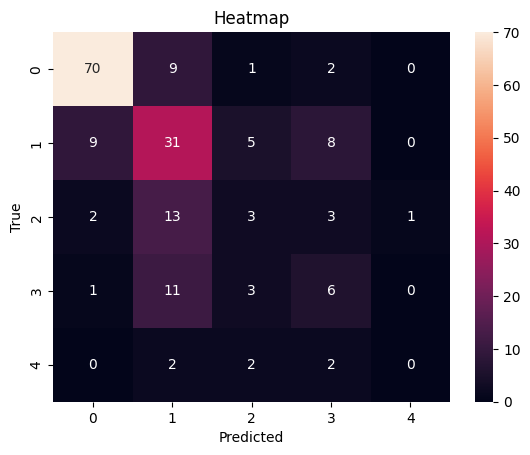
\includegraphics[width=0.75\linewidth]{rysunki/heart/macierz_pomylek_dnn_heart.png}
    \caption{Macierz pomyłek modelu sieci neuronowej dla zbioru dotyczącego choroby serca [źródło własne]}
    \label{fig:confusion_matrix_dnn_heart_disease}
\end{figure}

Na wykresie znajdującym się na Rys. \ref{fig:lime_barchar_dnn_heart} widać parę odznaczających się słupków. Najwyższym z nich jest ten odpowiadający kolumnie ,,oldpeak'' dla klasy '0' osiągającej istotność według metody \textbf{LIME} na poziomie ok. 0.16. Najistotniejszym czynnikiem stadium '1' okazał się ,,exang'' z wartością ponad 0.14. Wariant '3' miał bardzo wyraźne wskaźniki przewyższające te, wskazane dla osobników '2' klasy, a cechą najbardziej za nim przemawiającą było ,,fbs''. W tym drugim przypadku, jak i również ostatnim, ,,oldpeak'' okazało się być najistotniejsze. Zmienna ,,sex'' nie niosła za sobą żadnej istotnej przesłanki. 

\begin{figure}[H]
    \centering
    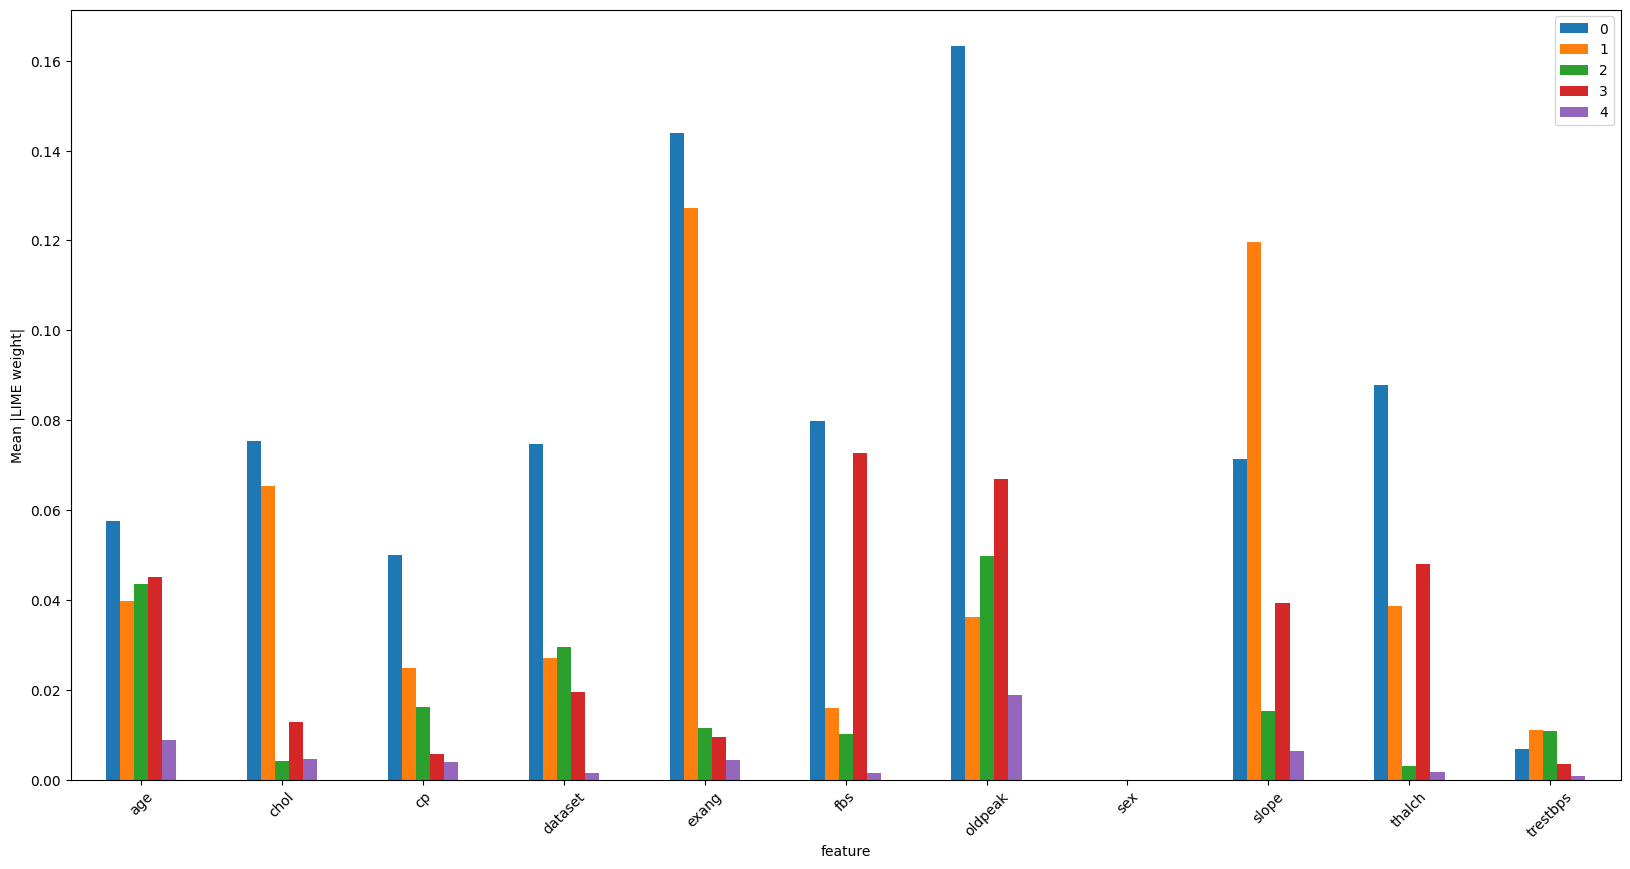
\includegraphics[width=0.9\linewidth]{rysunki/heart/lime_barchar_dnn_heart.png}
    \caption{Wykres słupkowy średnich wartości bezwzględnych wag LIME dla każdej z klasy modelu sieci neuronowej zbioru dotyczącego choroby serca [źródło własne]}
    \label{fig:lime_barchar_dnn_heart}
\end{figure}

Na Rys. \ref{fig:lime_absolutemeanplot_dnn_heart}, tak samo jak na poprzednim wykresie, najdłuższy okazuje się być ten słupek należący do ,,oldpeak'', tym razem z wartością ogólną wynoszącą ponad 0.065. Następne w rankingu znajduje się ,,exang'', a później ,,slope''. Na samym dole umieszczone zostało ,,sex'', które ma wagę 0. Nad nim widnieje ,,trestbps'', a trochę wyżej, ale z dużo lepszym wynikiem, mieści się ,,cp''.   

\begin{figure}[H]
    \centering
    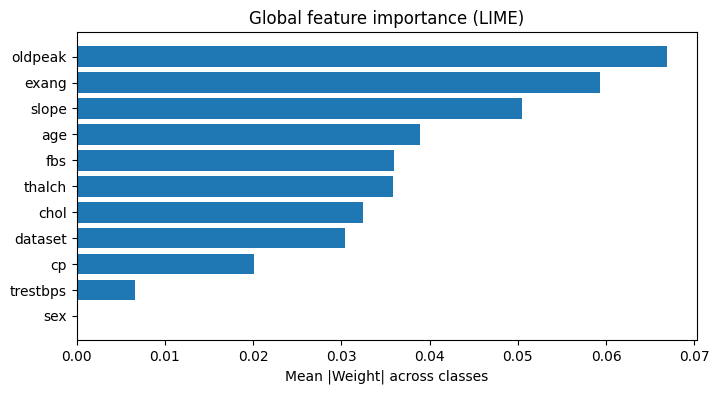
\includegraphics[width=0.75\linewidth]{rysunki/heart/lime_absolutemeanplot_dnn_heart.png}
    \caption{Wykres średnich obliczonych z bezwzględnych wartości wag LIME modelu sieci neuronowej zbioru dotyczącego choroby serca [źródło własne]}
    \label{fig:lime_absolutemeanplot_dnn_heart}
\end{figure}

Według wykresu metody \textbf{SHAP} zamieszczonego na Rys. \ref{fig:shap_barchar_dnn_heart} dla wariantu '0' najważniejszą przesłanką okazuje się być ,,cp'' z wartością 0.1, następnie ,,oldpeak'' z 0.08 i ,,exang'' z 0.07. W przypadku '1' najważniejszy jest ,,exang'', którego miara wynosi 0.06. Dla '2' doszło do ciekawej sytuacji, albowiem aż 3 cechy posiadają jednakowy wynik rzędu ok. 0.03 i są to ,,age'', ,,dataset'' i ,,cp''. ,,Oldpeak'' to najistotniejsza informacja predykcyjna '3' oraz '4' klasy. Prawie w każdym przypadku (oprócz '4') najmniej ważną przesłankę niosło za sobą ,,trestbps''.    

\begin{figure}[H]
    \centering
    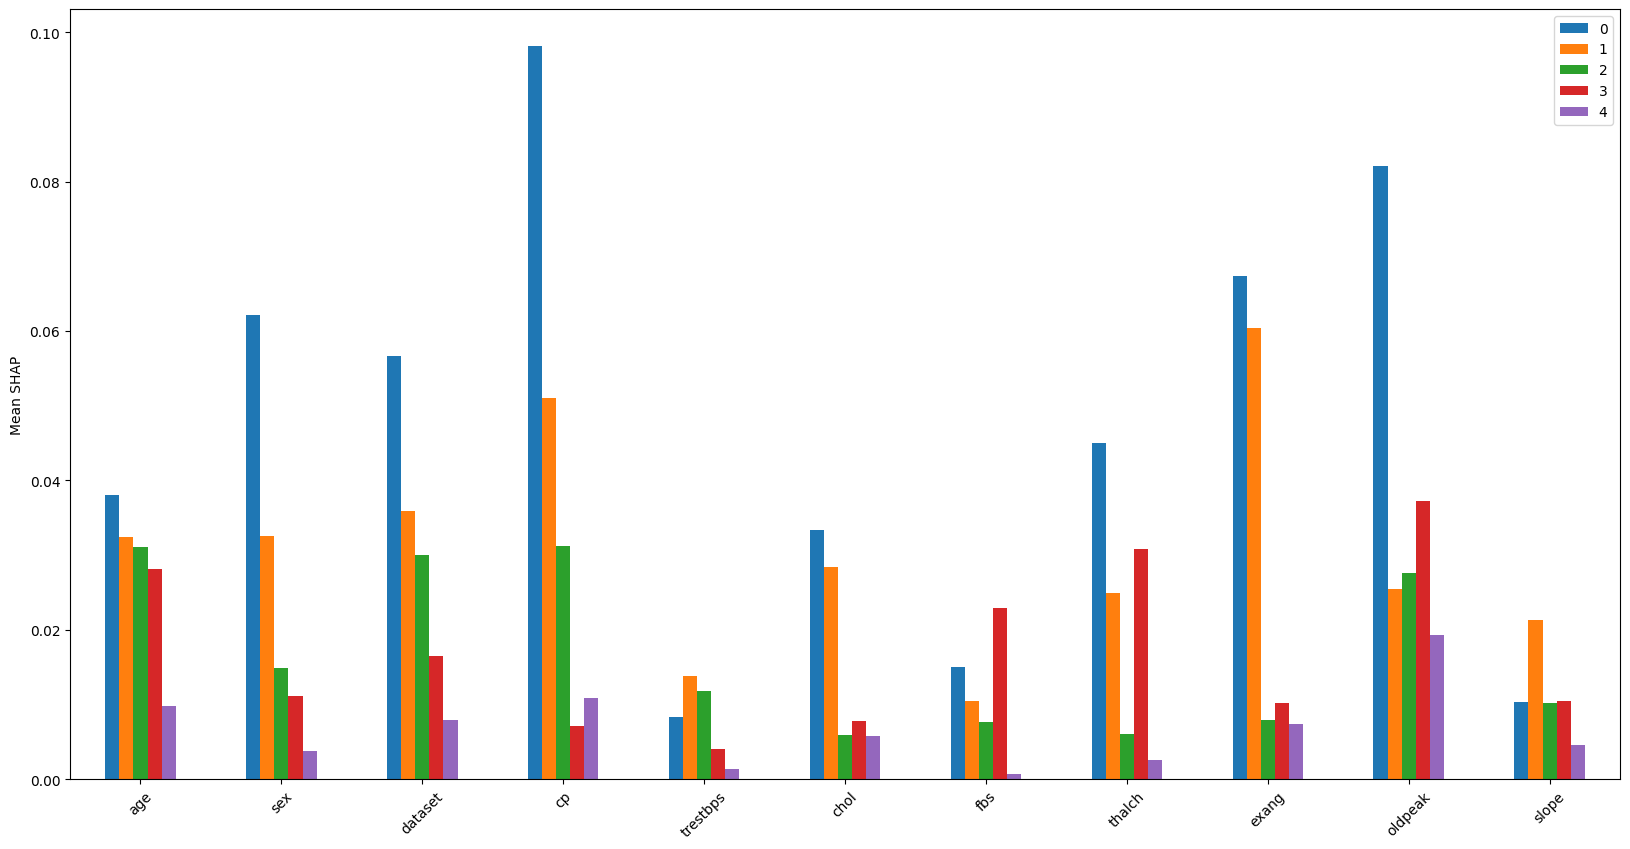
\includegraphics[width=0.9\linewidth]{rysunki/heart/shap_barchar_dnn_heart.png}
    \caption{Wykres słupkowy średnich wartości SHAP dla każdej z klasy modelu sieci neuronowej zbioru dotyczącego choroby serca [źródło własne]}
    \label{fig:shap_barchar_dnn_heart}
\end{figure}

Z wizualizacji przedstawionej na Rys. \ref{fig:shap_absolutemeanplot_dnn_heart} można wyczytać, że na przestrzeni wszystkich klas za najważniejszą cechę uznano ,,cp'' z wartością na poziomie 0.08. Następne w kolejności były predyktory ,,exang'' oraz ,,oldpeak'', które uzyskały wartość 0.06. Najmniej istotne okazały się być ,,slope'' i ,,trestbps'' przedstawione za pomocą sumy na samym dole. Ze względu na obcinanie liczb stojących na 3 miejscu po przecinku wykres początkowo może wydawać się błędny ze względu na napisane czerwoną czcionką miary znajdujące się po prawej stronie od słupków. Znajduje się tam parę wartości jednakowych, których słupki nie kończą się w tym samym miejscu. Wydaje się to być mylące.

\begin{figure}[H]
    \centering
    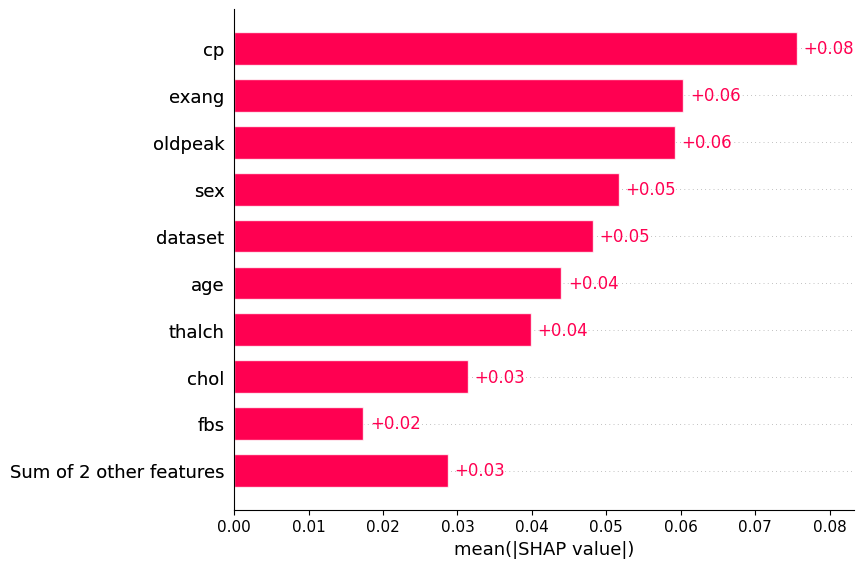
\includegraphics[width=0.75\linewidth]{rysunki/heart/shap_absolutemeanplot_dnn_heart.png}
    \caption{Wykres średnich obliczonych z bezwzględnych wartości SHAP modelu sieci neuronowej zbioru dotyczącego choroby serca [źródło własne]}
    \label{fig:shap_absolutemeanplot_dnn_heart}
\end{figure}

\iffalse
Jak widzimy z wykresu zaprezentowanego na Rys. \ref{fig:shap_beeswarm_dnn_heart} jeśli ,,cp'' jest niskie to jego wpływ oscyluje wokół -0.1 oraz 0.05, średnie to wokół 0.1, a duże przy -0.05 i od 0.1 do 0.3. Przy zmiennej ,,sex'' podział ten jest bardzo wyraźny, gdzie niskie wartości posiadają mały i zarazem duży wpływ, a wysokie mają znikomą istotność. Odwrotna sytuacja ma miejsce w przypadku ,,fbs''. Wyniki ,,age'' tworzą początkowo płynne przejście kolorystyczne, po czym dwa skrajne kolory zaczynają się ze sobą mieszać, tworząc niezbyt pomocną interpretację.

\begin{figure}[H]
    \centering
    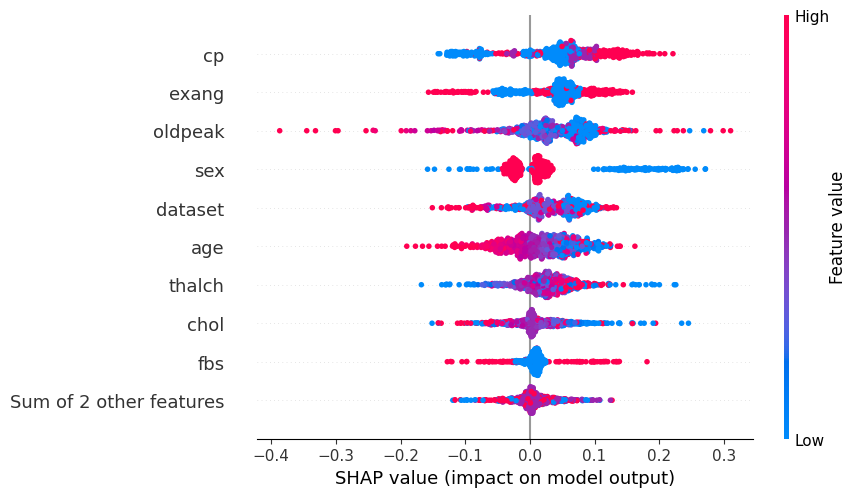
\includegraphics[width=1\linewidth]{rysunki/heart/shap_beeswarm_dnn_heart.png}
    \caption{Wykres typu ,,beeswarm'' wartości SHAP modelu sieci neuronowej zbioru dotyczącego choroby serca [źródło własne]}
    \label{fig:shap_beeswarm_dnn_heart}
\end{figure}
\fi

\begin{xltabular}{\textwidth}{|c|c|c|}
    \caption{Wyniki uzyskane po użyciu metody PFI przy modelu sieci neuronowej dla zbioru dotyczącego choroby serca}
    \label{tab:heart_disease_dnn_pfi}\\ \hline
    Cecha & Średnia & Odchylenie standardowe \\ \hline
    \endfirsthead
        oldpeak  & 0.053 &  0.011 \\ \hline
        dataset  & 0.045 &  0.008 \\ \hline
        exang    & 0.043 &  0.008 \\ \hline
        cp       & 0.041 &  0.009 \\ \hline
        age      & 0.036 &  0.009 \\ \hline
        thalch   & 0.029 &  0.008 \\ \hline
        fbs      & 0.027 &  0.006 \\ \hline
        chol     & 0.024 &  0.008 \\ \hline
        sex      & 0.022 &  0.008 \\ \hline
        slope    & 0.015 &  0.005 \\ \hline
        trestbps & 0.011 &  0.004 \\ \hline
\end{xltabular}

Wszystkie cechy zostały uznane przez \textbf{PFI} jako istotne, jednakże uzyskane przez nie wyniki są szczególnie niskie. Jak wskazuje Tabela \ref{tab:heart_disease_dnn_pfi} najważniejszym parametrem okazało się być ,,oldpeak'' ze spadkiem w dokładności na poziomie jedynie 5.3\% i odchyleniem standardowym 0.011. Na dalszych pozycjach znajduje się ,,dataset'' z wartością 4.5\%, a zaraz po nim ,,exang'' z 4.3\%. Za najmniej istotną przesłankę wskazano ,,trestbps'' z wynikiem wynoszącym 1.1\% i odchyleniem standardowym rzędu 0.004.

\begin{figure}[H]
    \centering
    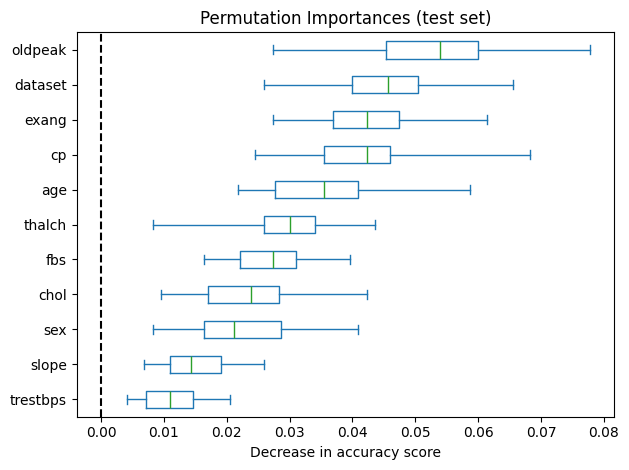
\includegraphics[width=0.75\linewidth]{rysunki/heart/pfi_dnn_heart.png}
    \caption{Wykres pudełkowy pokazujący wpływ cech na predykcję uzyskany po użyciu metody PFI przy modelu sieci neuronowej dla zbioru dotyczącego choroby serca [źródło własne]}
    \label{fig:box_plot_dnn_pfi}
\end{figure}

\subsubsection{Podsumowanie}
Wszystkie modele uczone i testowane na tych samych zbiorach pod względem dokladności uzyskały wyniki na przeciętnym poziomie. Były one do siebie zbliżone i oscylowały w granicach 60\%-64\%. Najlepiej pod tym względem poradził sobie XGBoost, jednak miał o około 1 jednostkę mniejsze ROC AUC od lasu losowego, u którego miara ta wyniosła 0.85. We wszystkich przypadkach najtrafniej diagnozowano klasę '0', przy czym najwięcej poprawnie należących do niej próbek, bo aż 70 z 82 wskazała sieć neuronowa, osiągając przy tym precyzję i czułość na poziomie 85\%. Podobnie decydowano o przynależności próbek do poszczególnych wariantów, z równą tendendcją spadkową, pogłębiającą się wraz z numerem przewidywanej kategorii. Wyniki większości średnich arytmetycznych były niezadowalające. Ich wartości ewidentnie wynikały z niezbilansowania danych, co możemy dostrzec analizując ilości rekordów dla poszczególnych klas znajdujące się w kolumnie 'Liczba'. Zauważamy wtedy, że liczebność zbioru testowego klasy '0' wyniosła 82 przypadki, a wariantu '4' jedynie 6. Z powodu tej ogromnej dysproporcji oraz niskiej zbiorowości prawie nigdy nie zaliczano próbek do najwyższej grupy ryzyka. Jeden raz, dla dwoch pierwszych modeli udało się jedną z nich poprawnie sklasyfikować, sieć neuronowa postawiła na błędną diagnozę o numerze '3'.  

Każdy z badanych modeli posiadał chociaż jeden atrybut, w którym był lepszy od innych. Jednak metryki, takie jak dokładność i średnia arytmetyczna, będące podatne na niezbilansowane dane, tracą na wiarygodności. Dlatego w przypadku tego zbioru lepiej jest kierować się innymi miarami. Uznano, że ze względu na sposób wyliczania najodpowiedniejsze będzie ROC AUC, pokazujące umiejętność rozróżniania pomiędzy poszczególnymi klasami. Ta idea plasuje las losowy na pierwszym miejscu. 

\begin{table}[H]
\centering
\caption{3 najistotniejsze oraz najmniej istotne cechy wskazane przez metody dla każdego z modeli w zbiorze dotyczącym choroby serca}
\label{tab:3_top_and_least_heart}
\begin{tabular}{|c|c|c|c|}
\hline
Model & Metoda & 3 najistotniejsze cechy & 3 najmniej istotne cechy \\ \hline
\multirow{3}{*}{Random Forest}& LIME& exang, oldpeak, age& trestbps, chol, sex\\ \cline{2-4} 
 & SHAP& cp, thalch, dataset& sex, fbs, slope\\ \cline{2-4} 
 & PFI& dataset, cp, age& sex, fbs, slope\\ \hline
\multirow{3}{*}{XGBoost}& LIME
& exang, cp, age& trestbps, thalch, sex\\ \cline{2-4} 
 & SHAP
& cp, thalch, age& sex, fbs, slope\\ \cline{2-4} 
 & PFI& age, oldpeak, chol& sex, fbs, slope\\ \hline
\multirow{3}{*}{Sieć neuronowa}& LIME
& oldpeak, exang, thalch& chol, trestbps, sex\\ \cline{2-4} 
 & SHAP
& age, cp, thalch& trestbps, slope, fbs\\ \cline{2-4} 
 & PFI& oldpeak, dataset, exang& sex, slope, trestbps \\ \hline
\end{tabular}
\end{table}

Jak możemy wyczytać z Tabeli \ref{tab:3_top_and_least_heart}  dla modelu Random Forest każda z metod wskazała inne 3 najistotniejsze cechy. LIME podała najbardziej odmienne zmienne, z których jedynie ,,age'' i ,,sex'' pojawiły się w innych wierszach należących do lasu losowego. SHAP i PFI były jednogłośne w kwestii najmniej znaczących przesłanek, czyli ,,,sex'', ,,fbs'' oraz ,,slope''. 

W przypadku XGBoost we wszystkich wytłumaczeniach wśród 3 najistotniejszych cech znalazło się ,,age'', a najmniej istotnych ,,sex''. Dwukrotnie pojawia się ,,cp'' - w 3 kolumnie dla LIME i SHAP. Co zastanawiające pierwsza z tych metod uznała ,,thalch'' za mało wartościowe, kiedy to druga w przeciwieństwie do niej umieściła tę zmienną bardzo wysoko w rankingu istotności. PFI wraz z wartościami Shapley'a był zgodny co do najmniej interesujących cech, wskazując już wcześniej wspomniane ,,sex'', ,,fbs'' oraz ,,slope''.

W sieci neuronowej wyjaśnienia były do siebie dosyć zbliżone. Wpośród 3 najmniej istotnych cech za każdym razem pojawiło się ,,trestbps'', z przeplatającym się ,,sex'' i ,,slope''. Natomiast wśród 3 najistotniejszych zmiennych nie pojawiła się jedna dominująca informacja, ale dwukrotnie znalazło się ,,oldpeak'', ,,exang'' oraz ,,thalch''.

W 8 na 9 przypadków za jednego z najmniej istotnych parametrów wskazano ,,sex'', nie pojawiła się ona wyłącznie w wytłumaczeniu SHAP dla sieci neuronowej, gdzie uznano ją za dosyć wartościową informację. Przy lesie losowym oraz XGBoost SHAP z PFI podawały identyczne wartości w 4 kolumnie. LIME bez względu na model zawsze za jedną z naistotniejszych cech podawał ,,exang'', a najmniej ważnych - ,,trestbps'' i ,,sex'', SHAP ,,cp'' z ,,thalch'', a także ,,fbs'' oraz ,,slope'', natomiast PFI nie miał faworyta w pierwszej kategorii, w drugiej - ,,sex'' i ,,slope''.


\subsection{Brain MRI Images for Brain Tumor Detection}
Jak możemy wyczytać z Tabeli \ref{tab:metrics_brain} model \textbf{VGG-16} uzyskał ROC AUC na poziomie 0.91. Zbiór testowy składał się jedynie z 26 obrazów. Do klasy decyzyjnej '0' należało 10, a '1' - 16. Spowodowało to niewielkie różnice pomiędzy średnią arytmetyczną a ważoną w postaci 1 punktu procentowego dla pierwszych miar. Precyzja, czułość i F1-score wyniosły 88\%, a specyficzność - 80\%. Dokładność modelu osiągnęła 85\%. Model poprawnie zaklasyfikował 8 z 10 obrazów bez zmian nowotworowych oraz 14 z 16 ze zmianami. Badany model z prawdopodobieństwem w przybliżeniu 100\% zaklasyfikował badaną próbkę jako wariant z guzem, co było poprawnym wyborem.

Model \textbf{ResNet50} osiągnął ROC AUC na poziomie 1.0. Precyzja wyniosła 94\%, a czułość - 100\%, co dało F1-score na poziomie 97\%, natomiast specyficzność osiągnęła 90\%. Średnie arytmetyczne i ważone omawianych miar oscylowały w przedziale od 95\% do 97\%. Model wykazał dokładność na poziomie 96\%. W klasyfikacji popełniony został tylko jeden błąd, a mianowicie jeden z przypadków klasy '0' został błednie oznaczony jako '1'. Badana próbka została poprawnie zdiagnozowana z praktycznie 100\% pewnością jako posiadająca zmiany nowotworowe.

\textbf{Xception} osiągnął ROC AUC na poziomie 0.99. Jego dokładność wyniosła 92\%. Precyzja wskazała 89\%, czułość była perfekcyjna i uzyskała 100\%, co skutkowało 94\% F1-score. Specyficzność była najmniejsza - z wynikiem 80\%. Dokładność modelu oceniono na 92\%. Jego średnie arytmetyczne i ważone opisanych wcześniej dla poszczególnych klas miar mieściły się w przedziale od 90\% do 94\%. Tylko 2 przypadki zostały źle zdiagnozowane. Stwierdzono na nich zmiany nowotworowe, gdy w rzeczywistości ich tam nie było. Badana próbka została poprawnie zaklasyfikowana jako posiadająca zmiany nowotworowe z prawdopodobieństwem bliskim 100\%. 


\begin{xltabular}{\textwidth}{|c|>{\centering\arraybackslash}X|c|c|c|c|c|}
\caption{Wyniki metryk poszczególnych modeli dla zbioru dotyczącego diabetyków}
\label{tab:metrics_brain}\\
\hline
Model \textbackslash Metryka & ROC AUC & Precyzja & Czułość & Specyficzność & F1-score & Dokładność \\ \hline
\endfirsthead
VGG-16 & 0.91 & 0.88 & 0.88 & 0.80 & 0.88 & 0.85 \\ \hline
ResNet50 & 1.0 & 0.94 & 1.0 & 0.90 & 0.97 & 0.96 \\ \hline
Xception & 0.99 & 0.89 & 1.0 & 0.80 & 0.94 & 0.92 \\ \hline
\end{xltabular}

\subsubsection{VGG-16}
Metoda \textbf{LIME} poprawnie wskazała dla badanej próbki klasę decyzyjną '1'. Na Rys. \ref{fig:lime_vgg16_1_brain} znajdują się 3 obrazki przedstawiające jej wytłumaczenia. Widzimy z niego, że wśród 5 najbardziej wpływowych obszarów nie znalazła się zmiana nowotworowa. Zostały zaznaczone części lewej strony obrazu, na których znajduje się kontur i leżące przy nim szare obszary. Pojawia się ona dopiero, gdy metoda podaje 10 najbardziej wpływowych superpikseli, zaraz obok dwóch rogów zdjęcia nie przedstawiających mózgu oraz oznaczonego na czerwono fragmentu nie zawierającego podejrzanych zmian. 

\begin{figure}[H]
    \centering
    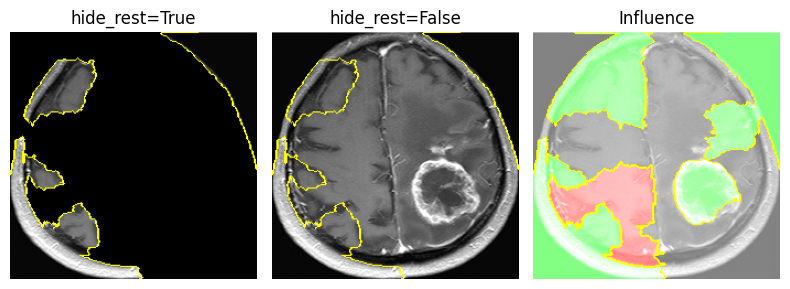
\includegraphics[width=0.9\linewidth]{rysunki/brain/lime_vgg16_1_brain.png}
    \caption{Wyniki uzyskane po zbadaniu próbki ze zmianami nowotworowymi za pomocą metody LIME dla modelu VGG-16 [źródło własne]}
    \label{fig:lime_vgg16_1_brain}
\end{figure}

\textbf{SHAP} poprawnie zaklasyfikował badaną próbkę jako zawierającą zmiany nowotworowe. Rys. \ref{fig:shap_vgg16_1_brain} przedstawia obrazki pokazujące jego wyjaśnienia. Na środkowym zdjęciu zauważamy, że metoda oznaczyła większą część obrazka jako przemawiającą za wskazaną klasyfikacją. Znajduje się w tym obszarze zmiana nowotworowa, jednak nasycenie koloru czerwonego nie wskazuje, żeby była najistotniejsza w przewidywaniu. Takim miejscem jest lewy dolny róg zdjęcia, który przedstawia kontur mózgu i obszar poza głową. Na przeciw diagnozie klasy '1' wychodzi znajdujący się zaraz obok kawałek oznaczony kolorem niebieskim. Ze zdjęcia zamieszczonego po lewej stronie dostrzegamy, że rzeczywiście nie widać na nim podejrzanych elementów. 

\begin{figure}[H]
    \centering
    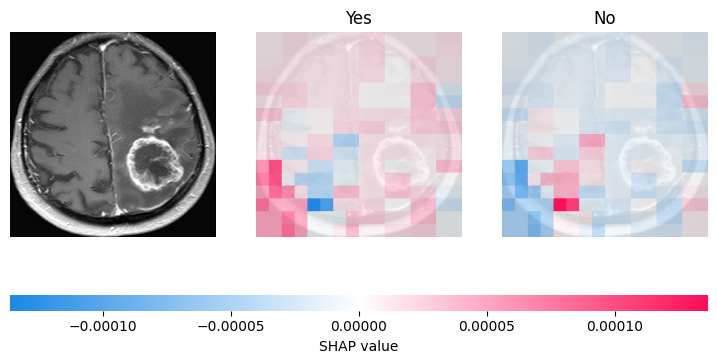
\includegraphics[width=0.9\linewidth]{rysunki/brain/shap_vgg16_1_brain.png}
    \caption{Wyniki uzyskane po zbadaniu próbki ze zmianami nowotworowymi za pomocą metody SHAP dla modelu VGG-16 [źródło własne]}
    \label{fig:shap_vgg16_1_brain}
\end{figure}

Na mapie stworzonej przy pomocy \textbf{Grad-CAM}, która znajduje się na Rys. \ref{fig:gradcam_vgg16_1_brain}, zostało zaznaczonych sporo obszarów. Wśród nich znajduje się zmiana nowotworowa, jednak jej oznaczenie zdaje się być trochę przesunięte wprawy dolny róg. Za najistotniejszy fragment metoda uznała lewą, środkową część obrazu przedstawiającą kontur mózgu i jego na szaro zaznaczone wnętrze poprzecinane ciemniejszymi liniami. W danej części nie widać jednak żadnych zmian nowotworowych. 

\begin{figure}[H]
    \centering
    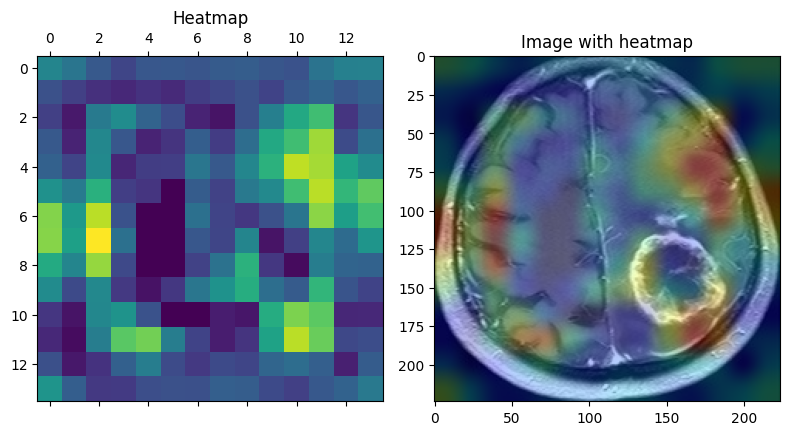
\includegraphics[width=0.65\linewidth]{rysunki/brain/gradcam_vgg16_1_brain.png}
    \caption{Wyniki uzyskane po zbadaniu próbki ze zmianami nowotworowymi za pomocą metody Grad-CAM dla modelu VGG-16 [źródło własne]}
    \label{fig:gradcam_vgg16_1_brain}
\end{figure}

\subsubsection{ResNet50}
\textbf{LIME} wyjaśniający działanie modelu ResNet50 poprawnie zdiagnozował badaną próbkę jako posiadającą zmiany nowotworowe. Z jego wytłumaczeń znajdujących się na Rys. \ref{fig:lime_resNet50_1_brain} możemy zauważyć, że pośród 5 najistotniejszych obszarów nie znalazł się ten z guzem. Metoda oznaczyła jedynie górną część zdjęcia oraz prawy środek zdjęcia, czyli fragment sąsiadujący z patologiczną częścią. Wśród 10 najbardziej wpływowych superpikseli już pojawiła się zmiana nowotworowa i nie wskazano żadnych elementów przeczących danej diagnozie. Zaistniały jednak obszary wykraczające poza kontur głowy. 

\begin{figure}[H]
    \centering
    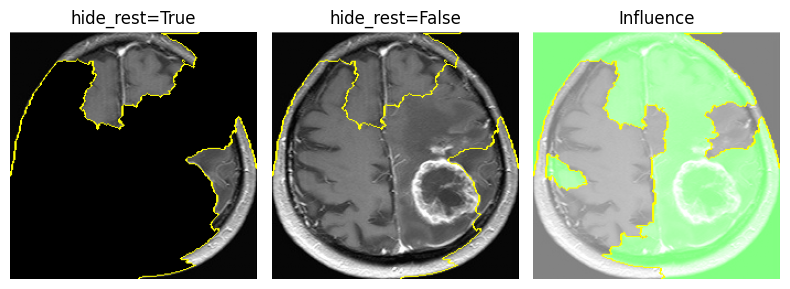
\includegraphics[width=0.9\linewidth]{rysunki/brain/lime_resNet50_1_brain.png}
    \caption{Wyniki uzyskane po zbadaniu próbki ze zmianami nowotworowymi za pomocą metody LIME dla modelu ResNet50 [źródło własne]}
    \label{fig:lime_resNet50_1_brain}
\end{figure}

Analizując wyjaśnienia \textbf{SHAP}, które znajdują się na Rys. \ref{fig:shap_resNet50_1_brain}, dostrzegamy, że guz mózgu został poprawnie oznaczony dosyć intensywnym czerwonym kolorem. Jednak nie jest najbardziej istotną częścią zdjęcia, albowiem według metody, owym elementem jest fragment konturu głowy znajdujący się w lewym górnym rogu oraz leżąca obok niego po prawej stronie część. Przeczące diagnozie elementy mieszczą się głównie na środku obrazka. Patrząc na oryginalne zdjęcie widzimy, iż nie ma tam niepożądanych zmian. 

\begin{figure}[H]
    \centering
    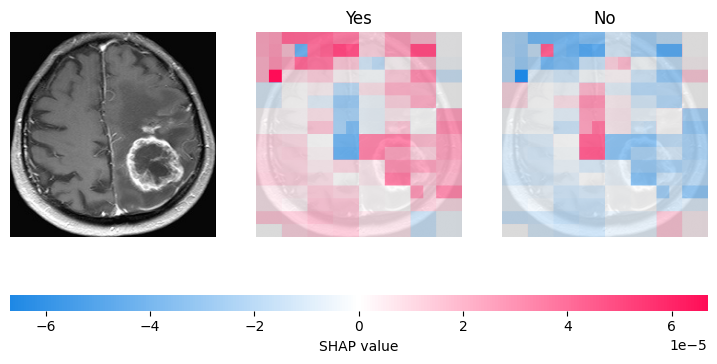
\includegraphics[width=0.9\linewidth]{rysunki/brain/shap_resNet50_1_brain.png}
    \caption{Wyniki uzyskane po zbadaniu próbki ze zmianami nowotworowymi za pomocą metody SHAP dla modelu ResNet50 [źródło własne]}
    \label{fig:shap_resNet50_1_brain}
\end{figure}

Na mapie stworzonej przy pomocy \textbf{Grad-CAM}, która znajduje się na Rys. \ref{fig:gradcam_resNet50_1_brain}, został wskazany tylko jeden obszar. Jest to znaleziona zmiana nowotworowa, jednak jej oznaczenie kieruje się bardziej do środka obrazka niż do samego guza. Dodatkowo kwadraty jakich użyto do zaznaczenia owego fragmentu są dosyć duże, przez co wyjaśnienie wydaje się być mało precyzyjne.

\begin{figure}[H]
    \centering
    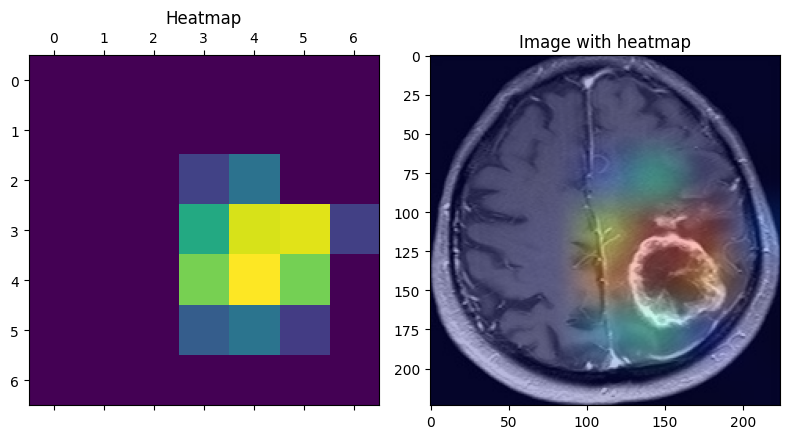
\includegraphics[width=0.65\linewidth]{rysunki/brain/gradcam_resNet50_1_brain.png}
    \caption{Wyniki uzyskane po zbadaniu próbki ze zmianami nowotworowymi za pomocą metody Grad-CAM dla modelu ResNet50   [źródło własne]}
    \label{fig:gradcam_resNet50_1_brain}
\end{figure}

\subsubsection{Xception}
Metoda \textbf{LIME} poprawnie zaklasyfikowała badaną próbkę jako klasę '1'. Jak możemy zauważyć na Rys. \ref{fig:lime_xception_1_brain}, wśród 5 najbardziej wpływowych obszarów znalazła się zmiana nowotworowa. Oprócz niej widnieją tam trzy fragmenty przedstawiające kontur głowy z czego jeden zawiera również szaro oznaczone wnętrze. Pośród 10 najistotniejszych przesłanek nie znalazła się żadna, która przeczyłaby danej diagnozie. Oprócz wcześniej wymienionych części pojawiły się tam trzy obszary znajdujące się poza głową, będące rogami zdjęcia.   

\begin{figure}[H]
    \centering
    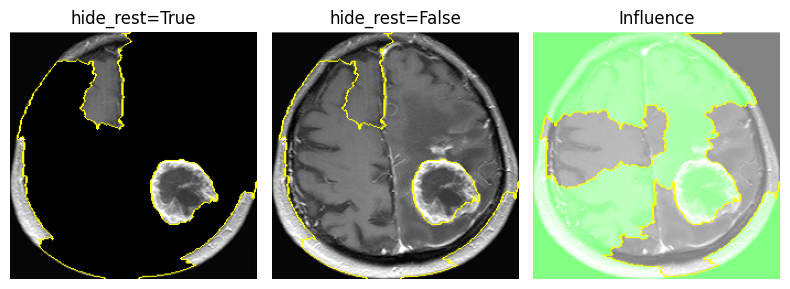
\includegraphics[width=0.9\linewidth]{rysunki/brain/lime_xception_1_brain.png}
    \caption{Wyniki uzyskane po zbadaniu próbki ze zmianami nowotworowymi za pomocą metody LIME dla modelu Xception   [źródło własne]}
    \label{fig:lime_xception_1_brain}
\end{figure}

\textbf{SHAP} poprawnie zdiagnozował badaną próbkę jako posiadającą patologiczne zmiany. Z Rys. \ref{fig:shap_xception_1_brain} możemy odczytać, że metoda zaznaczyła większą część zdjęcia jako istotną dla danej klasy decyzyjnej. Znalazł się tam fragment z guzem, a jego część odznaczała się intensywnie nasyconą czerwienią. Na zmianie nowotworowej znajdują się wyszarzone pola mówiące, że dane miejsce nie ma wartości predykcyjnej. Umieszczone zostały dwa niewielkie obszary przeczące danej predykcji - jeden mieszczący się w lewym dolnym rogu, a drugi pośrodku, bliżej prawej strony, przy samym krańcu zdjęcia. Są to części nieposiadające żadnych niepokojących elementów. 

\begin{figure}[H]
    \centering
    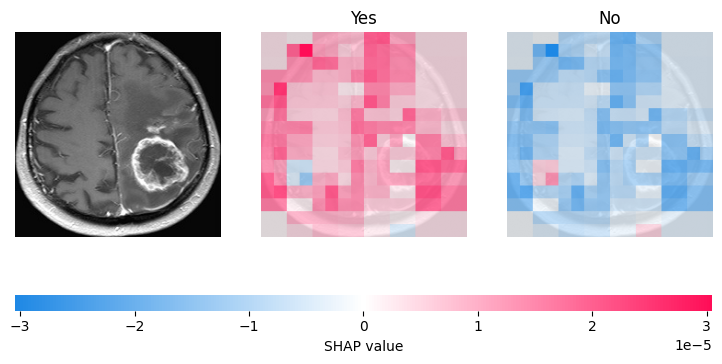
\includegraphics[width=0.9\linewidth]{rysunki/brain/shap_xception_1_brain.png}
    \caption{Wyniki uzyskane po zbadaniu próbki ze zmianami nowotworowymi za pomocą metody SHAP dla modelu Xception   [źródło własne]}
    \label{fig:shap_xception_1_brain}
\end{figure}

Jak widzimy na Rys. \ref{fig:gradcam_xception_1_brain} \textbf{Grad-CAM} wskazał jeden bardzo duży fragment zdjęcia. Znajduje się na nim guz, a jednemu z jego części przypisano jaskrawy żółty kolor, oznaczający wysoki, a nawet największy, wpływ na predykcję. Kwadraty użyte do oznaczania istotności poszczególnych części obrazu są sporawe, co prowadzi do ich mniejszej precyzji w próbie wyjaśnienia danej klasyfikacji. 

\begin{figure}[H]
    \centering
    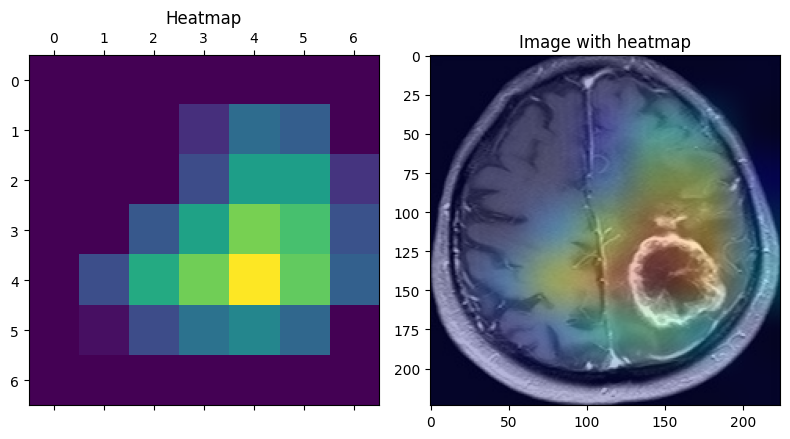
\includegraphics[width=0.65\linewidth]{rysunki/brain/gradcam_xception_1_brain.png}
    \caption{Wyniki uzyskane po zbadaniu próbki ze zmianami nowotworowymi za pomocą metody Grad-CAM dla modelu Xception   [źródło własne]}
    \label{fig:gradcam_xception_1_brain}
\end{figure}

\subsubsection{Podsumowanie}
Analizując wszystkie dostępne metryki, tj. ROC AUC, dokładność, precyzję, czułość i F1-score, najepiej ze wszystkich badanych modeli poradził sobie ResNet50. Popełnił on tylko jeden błąd na zbiorze testowym klasyfikując próbkę należącą w rzeczywistości do klasy decyzyjnej '1'. Najgorzej pod względem tych samych miar wypadł VGG-16 posiadający najprostszą architekturę. Odbiegał on od lidera o 11\% w poprawności swoich predykcji. Popełnił aż 4 błędy klasyfikując próbki zbioru testującego. Śmiem zatem twierdzić, że niestety nie najlepiej sprawdza się on w tak trudnym zadaniu jak wykrywanie zmian nowotworowych mózgu.

\begin{xltabular}{\textwidth}{|c|>{\centering\arraybackslash}X|c|>{\centering\arraybackslash}X|>{\centering\arraybackslash}X|}
\caption{Podsumowanie wyników uzyskanych przy badanej próbce posiadającej zmiany nowotworowe ze zbioru składającego się z rezonansów magnetycznych mózgów}
\label{tab:summary_brain}\\
\hline
Model & Prawdopodobień\-stwo nowotworu & Metoda & Czy w wyjaśnieniu występuje guz? & Czy w wyjaśnieniu znajduje się tło? \\ \hline
\endfirsthead
\multirow{3}{*}{VGG-16} & \multirow{3}{*}{100\%} & LIME & Tak* & Tak* \\ \cline{3-5} 
 &  & SHAP & Tak** & Tak \\ \cline{3-5} 
 &  & Grad-CAM & Tak** & Tak \\ \hline
\multirow{3}{*}{ResNet50} & \multirow{3}{*}{100\%} & LIME & Tak* & Tak* \\ \cline{3-5} 
 &  & SHAP & Tak & Tak \\ \cline{3-5} 
 &  & Grad-CAM & Tak & Nie \\ \hline
\multirow{3}{*}{Xception} & \multirow{3}{*}{99.67\%} & LIME & Tak & Tak* \\ \cline{3-5} 
 &  & SHAP & Tak & Tak** \\ \cline{3-5} 
 &  & Grad-CAM & Tak & Nie \\ \hline
\end{xltabular}

Dane zawarte w Tabeli \ref{tab:summary_brain} przedstawiają drobne podsumowanie wyników uzyskanych przez poszczególne metody dla modeli i badanej próbki. Odpowiedź ,,Tak*'' oznajmia - wystąpiło ale biorąc pod uwagę 10 najistotniejszych obszarów; a ,,Tak**'' - wystąpiło, ale nie było jedną z najważniejszych części fotografii. Z zaprezentowanych danych wynika, że biorąc pod uwagę częstotliwość występowania tła najlepszym wyborem byłby Grad-CAM, który tylko raz je oznaczył dla modelu VGG-16. Wracając jednak do jego szczegółowych wyników przypominamy sobie o wspomnianym problemie potencjalnie zbyt dużego i przez to mało precyzyjnego, obszaru wyjaśniającego. Kolejną w hierarchii wydaje się być metoda SHAP. Była ona jednak równie mało dokładna, często oznaczając dużą część zdjęcia, nierzadko mieszczącą się poza obrysem głowy. Pozostaje więc LIME, który w swoim tłumaczeniu zaznaczał bardzo szczegółowo fragmenty. Po rozszerzeniu przestrzeni rozwiązań do 10 obszarów pojawiał się wśród nich szukany guz i, niestety, rogi obrazu będące tłem. 


\subsection{Cats and Dogs Classification Dataset}
Z Tabeli \ref{tab:metrics_catsdogs} możemy odczytać, że model \textbf{VGG-16} osiągnął ROC AUC na poziomie 0.99. Precyzja, czułość, specyficzność i F1-score wyniosły odpowiednio 97\%, 96\%, 97\% i 97\%. Dokładność modelu oceniono na 97\%. Średnie aarytmetyczne i ważone ze względu na taki sam rozkład próbek względem klas decyzyjnych były jednakowe. Model poprawnie rozpoznał na 1940 z 2000 obrazach kota, a 1929 z 2000 psa. Tak niezwykle wysoka umiejętność klasyfikacji przełożyła się na fakt, że VGG-16 badanej próbce należącej do klasy '0' przypisał wartość 0.03, a do '1' - 1. Świadczy to o jego dużej pewności, co do wskazanych predykcji, które sa poprawne.

ROC AUC modelu \textbf{ResNet50} było perfekcyjne i osiągnęło 1.0. Precyzja, czułość, specyficzność i F1-score wyniosły 98\%. Taki sam wynik uzyskała także dokładność. Model poprawnie rozpoznał 1953 przypadki z 2000 przedstawiające kota poprawnie, a 1969 z 2000 obrazów psa. Próbka przynależąca do klasy '0' została zaklasyfikowana z 5\% prawdopodobieństwem do klasy przeciwnej, czyli model był niemal zupełnie pewny jej odmiennej diagnozy. Drugą ResNet50 ocenił na 99\% jako przeddstawiającą reprezentanta klasy '1'.

Wyniki modelu \textbf{Xception} są prawie idealne. Jego ROC AUC było na poziomie 1.0, a dokładność 99\%. Precyzja, czułość, specyficzność i F1-score osiągnęły odpowiednio 99\%, 99\%, 98\% i 99\%. Średnie arytmetyczne i ważone były identyczne. Model poprawnie sklasyfikował 1967 zdjęć kotów i 1976 psów z 2000 dostępnych dla obu klas. Pierwsza z badanych próbek zawierająca fotografię kota została oceniona na zaledwie 1\% jako przedstawiająca przeciwne w tym porówaniu stworzenie. Druga z nich została oceniona na 98\% jako reprezentantka klasy '1'. Przekłada się to na dużą pewność modelu co do jego predykcji.

\begin{xltabular}{\textwidth}{|c|>{\centering\arraybackslash}X|c|c|c|c|c|}
\caption{Wyniki metryk poszczególnych modeli dla zbioru dotyczącego diabetyków}
\label{tab:metrics_catsdogs}\\
\hline
Model \textbackslash Metryka & ROC AUC & Precyzja & Czułość & Specyficzność & F1-score & Dokładność \\ \hline
\endfirsthead
VGG-16 & 0.99 & 0.97 & 0.96 & 0.97 & 0.97 & 0.97 \\ \hline
ResNet50 & 1.0 & 0.98 & 0.98 & 0.98 & 0.98 & 0.98 \\ \hline
Xception & 1.0 & 0.98 & 0.99 & 0.98 & 0.99 & 0.99 \\ \hline
\end{xltabular}

\subsubsection{VGG-16}
Metoda \textbf{LIME} diagnozując badaną próbkę poprawnie wskazała jej przynależność do klasy '0'. Jak widzimy na Rys. \ref{fig:lime_vgg16_0_cats&dogs} wśród 5 najistotniejszych obszarów znalazł się kawałek główki kota, jego szyja oraz tło. Rozszerzenie przestrzeni do 10 najbardziej znaczących fragmentów poszerzyło wskazane wcześniej części o ich sąsiedztwo, czyli całą głowę, przestrzeń od szyji do połowy łapek, kark oraz kolejne części tła. Wśród nich nie znalazł się żaden, obszar przeczący danej klasyfikacji.

\begin{figure}[H]
    \centering
    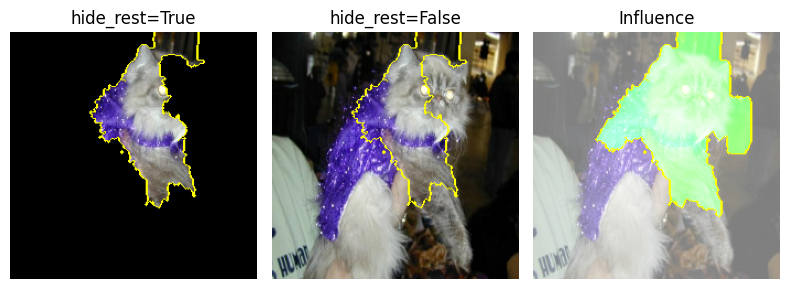
\includegraphics[width=0.9\linewidth]{rysunki/cats&dogs/lime_vgg16_0_cats&dogs.png}
    \caption{Wyniki uzyskane po zbadaniu próbki przedstawiającej kota za pomocą metody LIME dla modelu VGG-16 [źródło własne]}
    \label{fig:lime_vgg16_0_cats&dogs}
\end{figure}

Podobna sytuacj ma miejsce w przypadku próbki przedstawiającej pieska, która widnieje na Rys. \ref{fig:lime_vgg16_1_cats&dogs}. Tutaj \textbf{LIME} też poprawie zaklasyfikował obraz. Wśród 5 najbardziej wpływowych obszarów zaznaczył część pyszczka, a również kawałek łapki i udo z fragmentem ogona. Pośród 10 najistotniejszych cech znalazło się trochę tła obok kończyn stworzenia, przednia część torsu oraz większość tylnej lewej łapy. 

\begin{figure}[H]
    \centering
    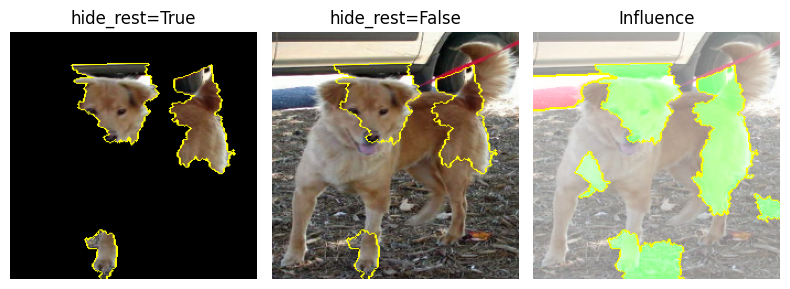
\includegraphics[width=0.9\linewidth]{rysunki/cats&dogs/lime_vgg16_1_cats&dogs.png}
    \caption{Wyniki uzyskane po zbadaniu próbki  przedstawiającej psa za pomocą metody LIME dla modelu VGG-16 [źródło własne]}
    \label{fig:lime_vgg16_1_cats&dogs}
\end{figure}

Analizując wyjaśnienia \textbf{SHAP} dla badanych próbek, które znajdują się na Rys. \ref{fig:shap_vgg16_0_cats&dogs} i \ref{fig:shap_vgg16_1_cats&dogs}, poprawnie zaklasyfikowane przez metodę, możemy zauważyć, że w dużej mierze wskazują one na ciała zwierząt. Szczególnie widać to w przypadku kota. Niestety zaznaczona została też część tła. W przypadku mruczka najważniejszym wskazanym fragmentem okazuje się być jego tylna część grzbietu, a wyjaśnienie pieska koncentruje się w znacznym stopniu na pyszczku. Niebieska część znajduje się w lewym dolnym rogu, w którym widnieje tył zwierzęcia. Na wersji ze szczekającym czworonogiem takie elementy są porozrzucane po całym zdjęciu, wskazując na tło, kawałek ogona czy łapy.     

\begin{figure}[H]
    \centering
    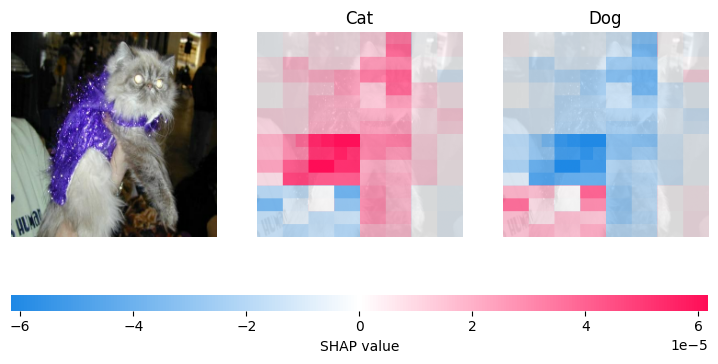
\includegraphics[width=0.9\linewidth]{rysunki/cats&dogs/shap_vgg16_0_cats&dogs.png}
    \caption{Wyniki uzyskane po zbadaniu próbki  przedstawiającej kota za pomocą metody SHAP dla modelu VGG-16 [źródło własne]}
    \label{fig:shap_vgg16_0_cats&dogs}
\end{figure}

\begin{figure}[H]
    \centering
    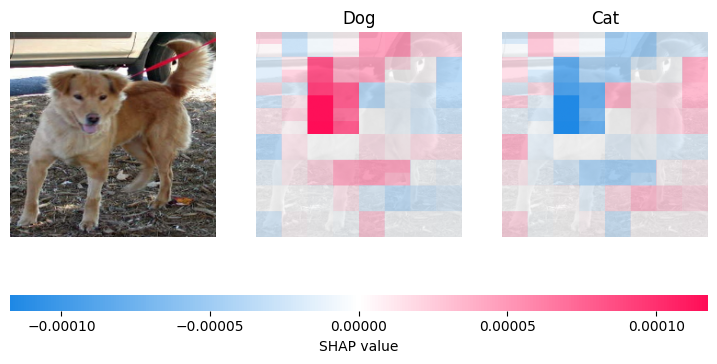
\includegraphics[width=0.9\linewidth]{rysunki/cats&dogs/shap_vgg16_1_cats&dogs.png}
    \caption{Wyniki uzyskane po zbadaniu próbki przedstawiającej psa za pomocą metody SHAP dla modelu VGG-16 [źródło własne]}
    \label{fig:shap_vgg16_1_cats&dogs}
\end{figure}

Analizując wyjaśnenia \textbf{Grad-CAM} widniejące na Rys. \ref{fig:gradcam_vgg16_0_cats&dogs} i Rys. \ref{fig:gradcam_vgg16_1_cats&dogs}, dostrzegamy, że w przypadku próbki z kotem metoda wskazała bardzo nikłe obszary. Znajdują się na nich tło, kawałek górnej części pyszczka oraz fragment torsu zwierzęcia. Lepiej w tym zadaniu poradził sobie z drugim obrazem, gdzie wyraźnie oznaczył pysk stworzenia w szczególności oczy oraz dodatkowo, ale już mniej intensywnie, tors, przednie łapy i końcówkę ogona.

\begin{figure}[H]
    \centering
    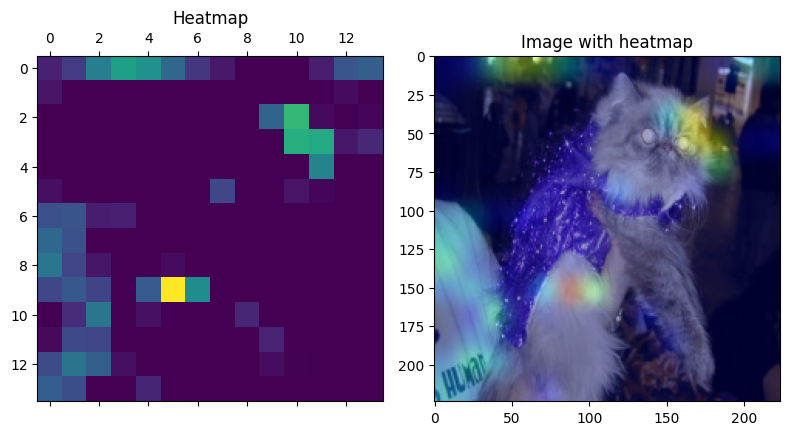
\includegraphics[width=0.65\linewidth]{rysunki/cats&dogs/gradcam_vgg16_0_cats&dogs.png}
    \caption{Wyniki uzyskane po zbadaniu próbki  przedstawiającej kota za pomocą metody Grad-CAM dla modelu VGG-16 [źródło własne]}
    \label{fig:gradcam_vgg16_0_cats&dogs}
\end{figure}

\begin{figure}[H]
    \centering
    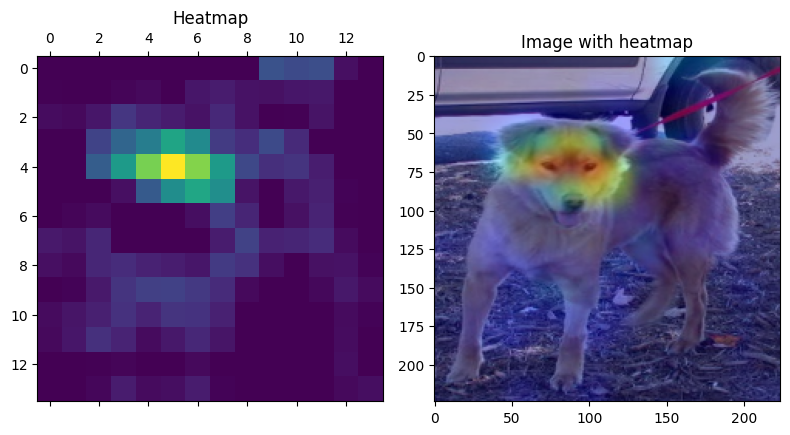
\includegraphics[width=0.65\linewidth]{rysunki/cats&dogs/gradcam_vgg16_1_cats&dogs.png}
    \caption{Wyniki uzyskane po zbadaniu próbki przedstawiającej psa za pomocą metody Grad-CAM dla modelu VGG-16   [źródło własne]}
    \label{fig:gradcam_vgg16_1_cats&dogs}
\end{figure}

\subsubsection{ResNet50}
\textbf{LIME} diagnozując próbkę z kotem poprawnie ją zaklasyfikował. Rozpatrując jego wyjaśnienia zamieszczone na Rys. \ref{fig:lime_resNet50_0_cats&dogs} spostrzegamy, że oznaczył on część głowy kota wycinając prawy fragment od nosa do policzka, a także bluzkę osoby trzymającej zwierzę z kawałkiem stroju w jaki zostało ono ubrane. Prawdopodobnie metoda mogła pomylić biały materiał z ogonem stworzenia, które ma podobne umaszczenie. Wśród 10 najbardziej wpływowych obszarów znalazło się wiele czerwonych plam, które zostały umiejscowione na łapach, szyi i części tła. Z pozytywnych elementów została usunięta lewa strona pyszczka i pozostała tylko ta górna. W przypadku próbki z psem, również dobrze sklasyfikowanej, przedstawionej na Rys. \ref{fig:lime_resNet50_1_cats&dogs}, LIME wskazał łapy zwierzęcia, górną część głowy i znajdujące się nad nią tło przedstawiające prawdopodobnie samochód. Rozszerzenie przestrzeni rozwiązań do 10 obszarów dodało do tłumaczenia więcej fragmentów scenerii, a także końcówkę ogona.

\begin{figure}[H]
    \centering
    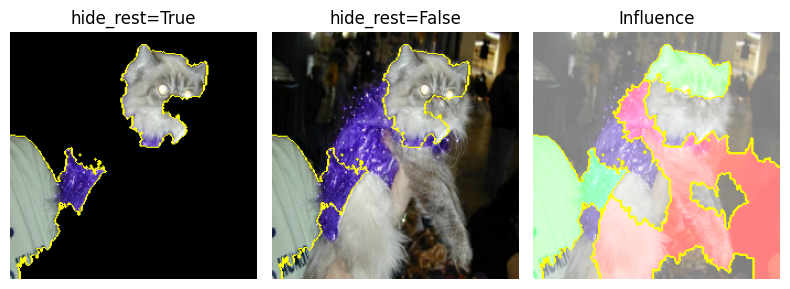
\includegraphics[width=0.9\linewidth]{rysunki/cats&dogs/lime_resNet50_0_cats&dogs.png}
    \caption{Wyniki uzyskane po zbadaniu próbki  przedstawiającej kota za pomocą metody LIME dla modelu ResNet50 [źródło własne]}
    \label{fig:lime_resNet50_0_cats&dogs}
\end{figure}

\begin{figure}[H]
    \centering
    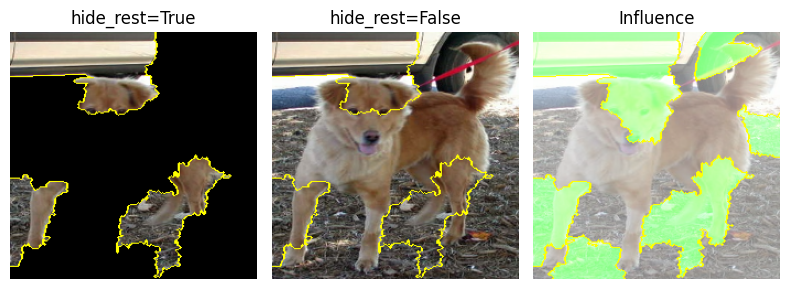
\includegraphics[width=0.9\linewidth]{rysunki/cats&dogs/lime_resNet50_1_cats&dogs.png}
    \caption{Wyniki uzyskane po zbadaniu próbki przedstawiającej psa za pomocą metody LIME dla modelu ResNet50 [źródło własne]}
    \label{fig:lime_resNet50_1_cats&dogs}
\end{figure}

\textbf{SHAP} jak wynika z zaprezentowanych Rys. \ref{fig:shap_resNet50_0_cats&dogs} i \ref{fig:shap_resNet50_1_cats&dogs} skupił się głównie na elementach pyszczków zwierząt. Dla kota oznaczył bardzo intensywnym czerwonym kolorem jego oczy z czołem, a psa nos i policzek. Oprócz nich pojawiło się wiele innych pozytywnie wpływających na predykcję fragmentów, jednak w przypadku pierwszego obrazu były one porozrzucane po całym zdjęciu, często wskazując na tło, a w drugim - znajdowały się po lewej stronie zdjęcia, z równą częstotliwością trafiając na scenerię. Analizując fotografię mruczka zauważamy porównywalnie wiele niebieskich obszarów, jednak żaden nie odznaczał się wyjątkową intensywnością. U psa elementów takich było niewiele i one również blakły na tle ich przeciwieństw.

\begin{figure}[H]
    \centering
    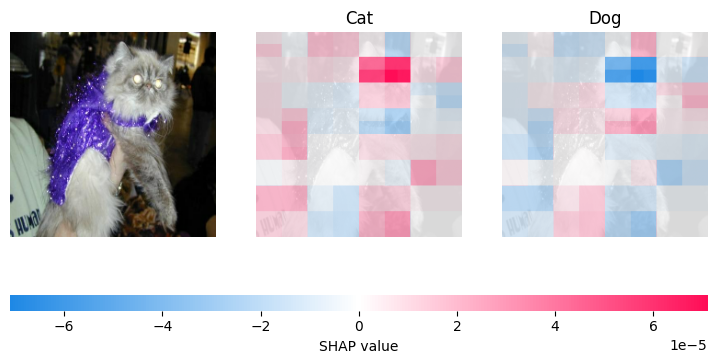
\includegraphics[width=0.9\linewidth]{rysunki/cats&dogs/shap_resNet50_0_cats&dogs.png}
    \caption{Wyniki uzyskane po zbadaniu próbki  przedstawiającej kota za pomocą metody SHAP dla modelu ResNet50 [źródło własne]}
    \label{fig:shap_resNet50_0_cats&dogs}
\end{figure}

\begin{figure}[H]
    \centering
    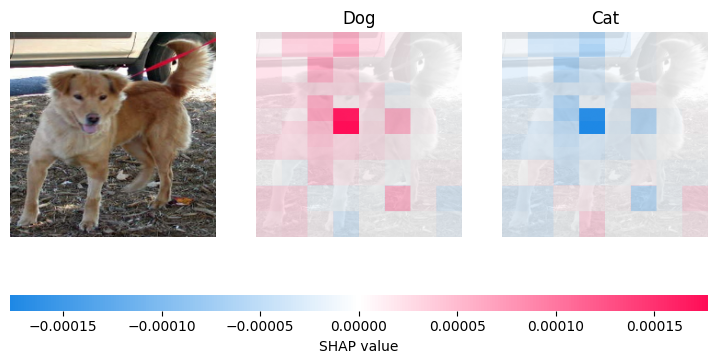
\includegraphics[width=0.9\linewidth]{rysunki/cats&dogs/shap_resNet50_1_cats&dogs.png}
    \caption{Wyniki uzyskane po zbadaniu próbki przedstawiającej psa za pomocą metody SHAP dla modelu ResNet50 [źródło własne]}
    \label{fig:shap_resNet50_1_cats&dogs}
\end{figure}

Obserwując zamieszcozne na Rys. \ref{fig:gradcam_resNet50_0_cats&dogs} i \ref{fig:gradcam_resNet50_1_cats&dogs} wyjaśnienia \textbf{Grad-CAM} dostrzegamy, że metoda wskazała w obydwu przypadkach dwa duże fragmenty zdjęć. Epicentrum kolorystyczne znalazło się na szyi kota oraz tylnej części torsu psa. Bardziej trafnym oznaczeniem wydaje się być to, osiągnięte przy fotografii psa, gdzie trochę mniej istotnym w danej metryce kolorem oznaczono resztę tłowia stworzenia z kawałkiem jego głowy. 

\begin{figure}[H]
    \centering
    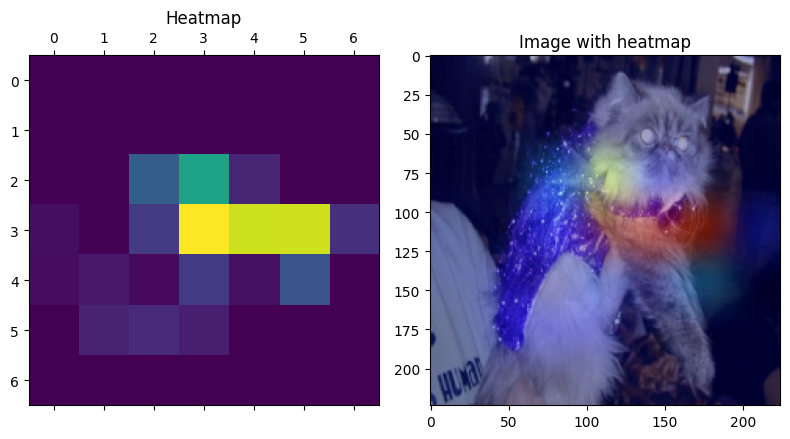
\includegraphics[width=0.65\linewidth]{rysunki/cats&dogs/gradcam_resNet50_0_cats&dogs.png}
    \caption{Wyniki uzyskane po zbadaniu próbki  przedstawiającej kota za pomocą metody Grad-CAM dla modelu ResNet50 [źródło własne]}
    \label{fig:gradcam_resNet50_0_cats&dogs}
\end{figure}

\begin{figure}[H]
    \centering
    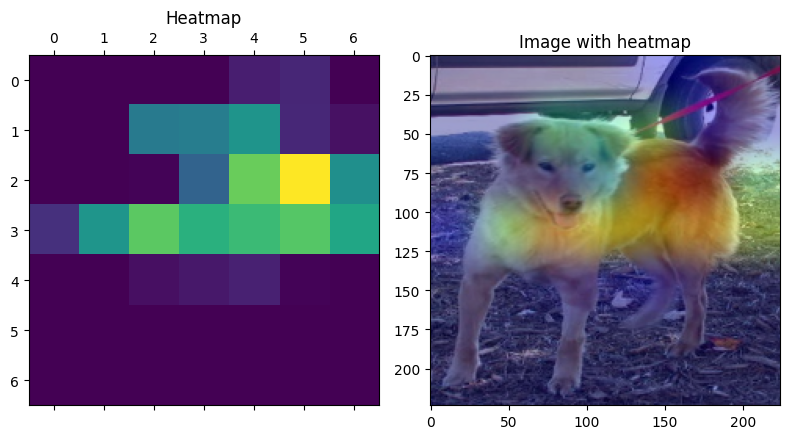
\includegraphics[width=0.65\linewidth]{rysunki/cats&dogs/gradcam_resNet50_1_cats&dogs.png}
    \caption{Wyniki uzyskane po zbadaniu próbki przedstawiającej psa za pomocą metody Grad-CAM dla modelu ResNet50 [źródło własne]}
    \label{fig:gradcam_resNet50_1_cats&dogs}
\end{figure}

\subsubsection{Xception}
Metoda \textbf{LIME} w swoich poprawnie sklasyfikowanym wytłumaczeniu, mieszczącym się na Rys. \ref{fig:lime_xception_0_cats&dogs}, doskonale wyodrębniła głowę kota i wskazała ją jako jeden z najwazniejszych obszarów predykcyjnych. Obok niej znalazło się także udo zwierzęcia. Wśród 10 najbardziej wpływowych fragmentów, oprócz tych wcześniej wskazanych znalazła się bluzka osoby trzymajacej stworzenie, jego przednie łapy oraz tło, z czego te dwa ostatnie obszary były zaznaczone na czerwono. W przypadku również dobrze sklasyfikowanego psa, którego tłumaczenie znalazło się na Rys. \ref{fig:lime_xception_1_cats&dogs}, \textbf{LIME} zwróciło najpierw uwagę na jego prawy dolny skrawek pyszczka oraz części przedniej i tylnej łapy. Rozszerzając przestrzeń rozwiązań do tłumaczenia dołączone zostało tło pomiędzy wspomnianymi już kończynami oraz kolejny fragment głowy zwierzęcia.  

\begin{figure}[H]
    \centering
    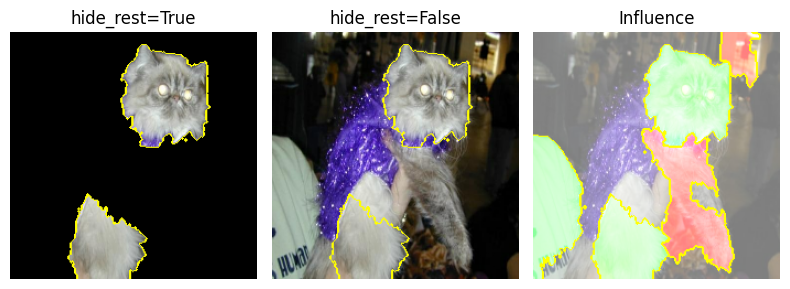
\includegraphics[width=0.9\linewidth]{rysunki/cats&dogs/lime_xception_0_cats&dogs.png}
    \caption{Wyniki uzyskane po zbadaniu próbki  przedstawiającej kota za pomocą metody LIME dla modelu Xception [źródło własne]}
    \label{fig:lime_xception_0_cats&dogs}
\end{figure}

\begin{figure}[H]
    \centering
    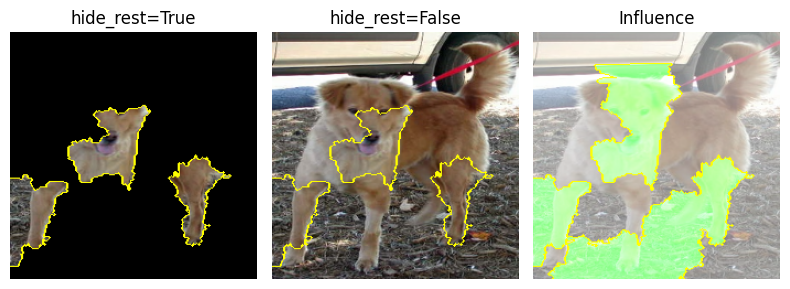
\includegraphics[width=0.9\linewidth]{rysunki/cats&dogs/lime_xception_1_cats&dogs.png}
    \caption{Wyniki uzyskane po zbadaniu próbki przedstawiającej psa za pomocą metody LIME dla modelu Xception [źródło własne]}
    \label{fig:lime_xception_1_cats&dogs}
\end{figure}

Patrząc na Rys. \ref{fig:shap_xception_0_cats&dogs} i \ref{fig:shap_xception_1_cats&dogs} widzimy, że \textbf{SHAP} w zadaniu klasyfikacji w dużej mierze kierował się głowami czworonogów, które odznaczały się największą intensywnością koloru czerwonego. Kolejnymi ważnymi w pozytywnym aspekcie w odpowiadających im przewidywaniach była reszta ciała stworzeń. Niestety wśród czerwonych punktów znalazło się też trochę tła. Niebieskie kwadraty o wiele bardziej rzucały się w oczy w przypadku zdjęcia z kotem niż z psem. W obu wariantach wskazywały one jednak głównie scenerię, a nie elementy czworonogów.  

\begin{figure}[H]
    \centering
    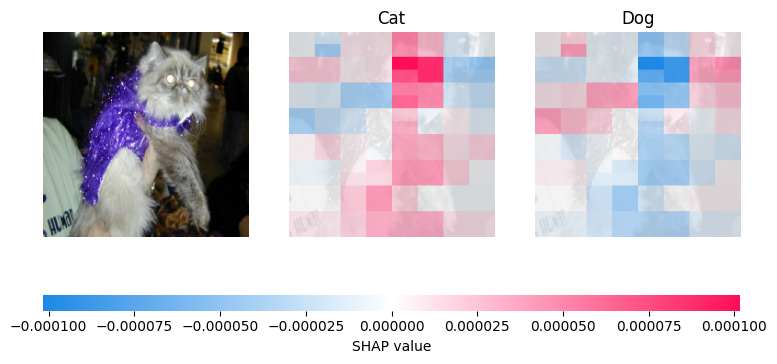
\includegraphics[width=0.9\linewidth]{rysunki/cats&dogs/shap_xception_0_cats&dogs.png}
    \caption{Wyniki uzyskane po zbadaniu próbki  przedstawiającej kota za pomocą metody SHAP dla modelu Xception [źródło własne]}
    \label{fig:shap_xception_0_cats&dogs}
\end{figure}

\begin{figure}[H]
    \centering
    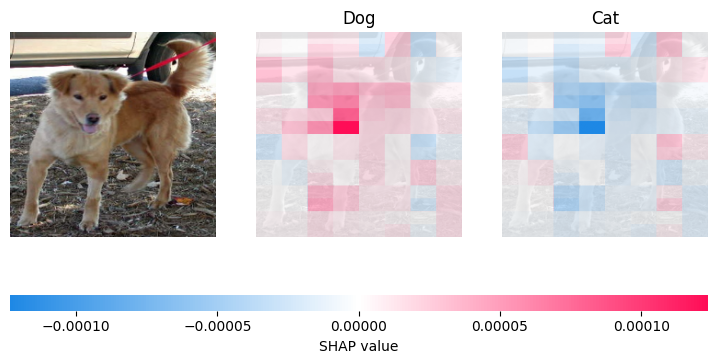
\includegraphics[width=0.9\linewidth]{rysunki/cats&dogs/shap_xception_1_cats&dogs.png}
    \caption{Wyniki uzyskane po zbadaniu próbki przedstawiającej psa za pomocą metody SHAP dla modelu Xception [źródło własne]}
    \label{fig:shap_xception_1_cats&dogs}
\end{figure}

\textbf{Grad-CAM}, jak zwracamy uwagę na Rys. \ref{fig:gradcam_xception_0_cats&dogs} i \ref{fig:gradcam_xception_1_cats&dogs}, kierował się wyjątkowo dużymi punktami w celu wytłumaczenia odpowiadającym im diagnoz, co prowadzi do sceptycznego spojrzenia na jego dokładność. W przypadku kota najintensywniejszym miejscem okazała się być tylna część grzbietu, od której w postaci swego rodzaju gradientu odchodziły mniej istotne fragmenty. Natomiast na obrazku przedstawiającym psa oznaczona została lewa oraz górna część fotografii, gdzie jej epicentrum znalazło się pośrodku. Znajdowało się pod tym tło oraz głowa z przodem torsu i znajdującymi się pod nim łapami. 

\begin{figure}[H]
    \centering
    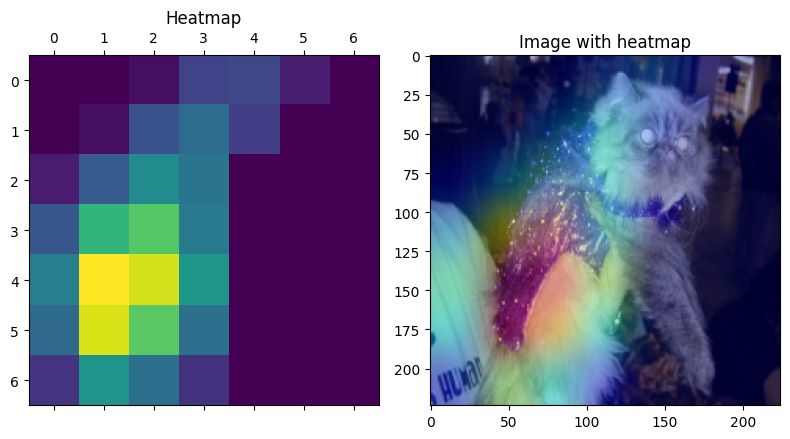
\includegraphics[width=0.65\linewidth]{rysunki/cats&dogs/gradcam_xception_0_cats&dogs.png}
    \caption{Wyniki uzyskane po zbadaniu próbki  przedstawiającej kota za pomocą metody Grad-CAM dla modelu Xception [źródło własne]}
    \label{fig:gradcam_xception_0_cats&dogs}
\end{figure}

\begin{figure}[H]
    \centering
    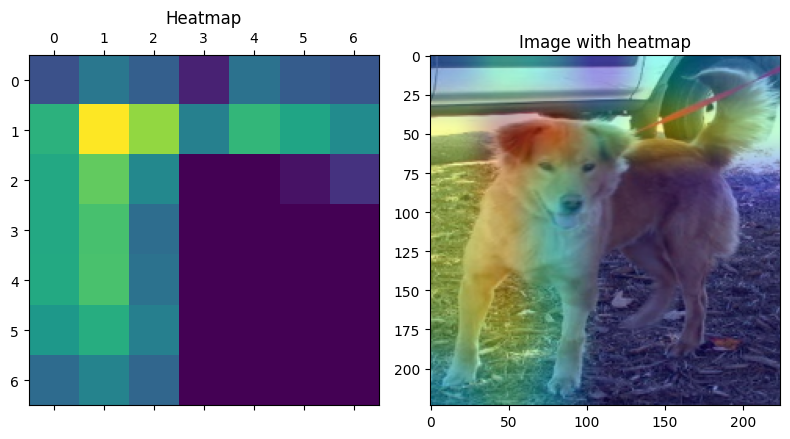
\includegraphics[width=0.65\linewidth]{rysunki/cats&dogs/gradcam_xception_1_cats&dogs.png}
    \caption{Wyniki uzyskane po zbadaniu próbki przedstawiającej psa za pomocą metody Grad-CAM dla modelu Xception [źródło własne]}
    \label{fig:gradcam_xception_1_cats&dogs}
\end{figure}

\subsubsection{Podsumowanie}
Sieci konwolucyjnie poradziły sobie znakomicie w rozpoznawaniu kotów i psów, a każda z nich osiągnęła dokładność większą, bądź równą, 97\%. Najlepiej w tym zadaniu klasyfikacyjnym popradził sobie pod względem wszystkich metryk Xception, chociaż inne modele były od niego minimalnie gorsze. Łącznie zrobił on tylko 57 błędów przydzielając poszczególne klasy próbkom. Najgorszy okazał się być VGG-16, ale pamiętając, że jest najprostszym architektonicznie rozwiązaniem, to trzeba uznać, iż wypadł on świetnie.  

\begin{xltabular}{\textwidth}{|c|>{\centering\arraybackslash}X|c|>{\centering\arraybackslash}X|>{\centering\arraybackslash}X|}
\caption{Podsumowanie wyników uzyskanych przy badanej próbce przedstawiającej kota ze zbioru dotyczącego klasyfikacji kotów i psów}
\label{tab:summary_0_catsdogs}\\
\hline
Model & Prawdopodobień\-stwo, że na zdjęciu jest pies & Metoda & Czy w wyjaśnieniu występuje pysk? & Czy w wyjaśnieniu znajduje się tło? \\ \hline
\endfirsthead
\multirow{3}{*}{VGG-16} & \multirow{3}{*}{3.56\%} & LIME & Tak & Tak \\ \cline{3-5} 
 &  & SHAP & Tak** & Tak** \\ \cline{3-5} 
 &  & Grad-CAM & Tak** & Tak** \\ \hline
\multirow{3}{*}{ResNet50} & \multirow{3}{*}{5.8\%} & LIME & Tak & Tak \\ \cline{3-5} 
 &  & SHAP & Tak & Tak** \\ \cline{3-5} 
 &  & Grad-CAM & Tak** & Tak** \\ \hline
\multirow{3}{*}{Xception} & \multirow{3}{*}{1.42\%} & LIME & Tak & Tak* \\ \cline{3-5} 
 &  & SHAP & Tak & Tak** \\ \cline{3-5} 
 &  & Grad-CAM & Tak** & Tak** \\ \hline
\end{xltabular}

\begin{xltabular}{\textwidth}{|c|>{\centering\arraybackslash}X|c|>{\centering\arraybackslash}X|>{\centering\arraybackslash}X|}
\caption{Podsumowanie wyników uzyskanych przy badanej próbce przedstawiającej psa ze zbioru dotyczącego klasyfikacji kotów i psów}
\label{tab:summary_1_catsdogs}\\
\hline
Model & Prawdopodobień\-stwo, że na zdjęciu jest pies & Metoda & Czy w wyjaśnieniu występuje pysk? & Czy w wyjaśnieniu znajduje się tło? \\ \hline
\endfirsthead
\multirow{3}{*}{VGG-16} & \multirow{3}{*}{100\%} & LIME & Tak & Tak \\ \cline{3-5} 
 &  & SHAP & Tak & Tak** \\ \cline{3-5} 
 &  & Grad-CAM & Tak & Tak** \\ \hline
\multirow{3}{*}{ResNet50} & \multirow{3}{*}{99.41\%} & LIME & Tak & Tak \\ \cline{3-5} 
 &  & SHAP & Tak & Tak** \\ \cline{3-5} 
 &  & Grad-CAM & Tak** & Tak** \\ \hline
\multirow{3}{*}{Xception} & \multirow{3}{*}{98.06\%} & LIME & Tak & Tak \\ \cline{3-5} 
 &  & SHAP & Tak & Tak** \\ \cline{3-5} 
 &  & Grad-CAM & Tak & Tak \\ \hline
\end{xltabular}

Analizując dane zawarte w Tabelach \ref{tab:summary_0_catsdogs} i \ref{tab:summary_1_catsdogs} dostrzegamy brak jakiejkolwiek odpowiedzi ,,Nie''. Napisy ,,Tak*'' oznacza, że obiekt pojawił się dopiero wśród 10 najistotniejszych obszarów, a ,,Tak**'' - nie był on najistotniejszy w zaprezentowanym tłumaczeniu. Wynika z tego, iż najgorzej poradził sobie Grad-CAM, w którego odpowiadających komórkach często widniały gwiazdki. Zaskakująco dobrze w owym zestawieniu wypada LIME dający najklarowniejsze wytłumaczenia i jeśli spojrzeć na poszczególne przypadki, najdokładniejsze. SHAP zaznaczał właściwe obszary jednak jego zakres odpowiedzi był zbyt obszerny i mało precyzyjny.
